%% comment out the first line before production.

\renewcommand{\thechapter}{3}
\chapter{Data Collection and Compilation}
\label{chap:data collection}

\begin{linenumbers}
\section{Water Quality Data Collection}
\label{sec:field data collection}

From June 2006 to July 2011 and April 2003 to August 2011, water quality samples were taken by CSU field personnel from the Arkansas River, tributaries, and drains in the USR and DSR, respectively.   During the Se study periods, 18 surface water sampling trips were made to the USR and 46 trips were made to the DSR.  A total of 288 dissolved Se samples were taken and analyzed for dissolved Se and specific ions in the USR and 1,030 in the DSR during their respective study periods.  Table \ref{tab:SampleSummary} is a summary of the sample trips, the month and year of the trip, and the number of Se samples taken from the respective locations.  Figures \ref{map:USRSample} and \ref{map:DSRSample} show the dissolved Se sample locations in the USR and DSR, respectively.  Tables \ref{tab:USRSampleLoc} and \ref{tab:DSRSampleLoc} list the sample locations and their location with the river reach and segment.  The location of the sample point within the segment is only listed for samples collected on the Arkansas River with respect to the location of the stream gauge within the river segment.  Sample points on tributaries and drains as noted in the tables.

% Table - sample trips
\afterpage{%
	\clearpage%
	\renewcommand{\arraystretch}{0.513}
	\begin{longtable}{c C{1.25in} C{.9in} C{1in} C{.9in} C{1in}}
		\caption[Summary of USR and DSR Water Sample Events.]{Summary of USR and DSR Water Sample Events.}    \label{tab:SampleSummary} \\
			\toprule
    	Trip & \multirow{2}[1]{*}{Date} & \multicolumn{2}{c}{USR Se Samples} & \multicolumn{2}{c}{DSR Se Samples} \\\cmidrule(r{.5em}l){3-4} \cmidrule(r{.5em}l){5-6}
    	\# &  & River & Trib. \& Drain & River & Trib. \& Drain \\
    		\toprule
    	\endfirsthead
    	\caption[]{Summary of USR and DSR Water Sample Events.  (Continued)}\\
    		\toprule
    	Trip & \multirow{2}{*}{Date} & \multicolumn{2}{c}{USR Se Samples} & \multicolumn{2}{c}{DSR Se Samples} \\
    	\# &  & River & Trib. \& Drain & River & Trib. \& Drain \\
    		\toprule
    	\endhead
    		\bottomrule
    	\endfoot 
		1 & April 2003 &  &  & 12 & 14 \\
		2 & June 2003 &  &  & 12 & 15 \\
		3 & July 2003 &  &  & 7 & 15 \\
		4 & July 2003 &  &  & 6 & 16 \\
		5 & October 2003 &  &  & 6 & 15 \\
		6 & January 2004 &  &  & 6 & 15 \\
		7 & March 2004 &  &  & 6 & 15 \\
		8 & May 2004 &  &  & 6 & 15 \\
		9 & June 2004 &  &  & 6 & 15 \\
		10 & July 2004 &  &  & 6 & 15 \\
		11 & August 2004 &  &  & 6 & 15 \\
		12 & November 2004 &  &  & 6 & 17 \\
		13 & January 2005 &  &  & 6 & 15 \\
		14 & March 2005 &  &  & 6 & 15 \\
		15 & June 2005 &  &  & 6 & 17 \\
		16 & July 2005 &  &  & 6 & 15 \\
		17 & August 2005 &  &  & 6 & 17 \\
		18 & December 2005 &  &  & 6 & 16 \\
		19 & January 2006 &  &  & 6 & 16 \\
		20 & March 2006 &  &  & 6 & 16 \\
		21 & May 2006 &  &  & 6 & 16 \\
		22 & June 2006 & 10 & 5 & 6 & 16 \\
		23 & July 2006 &  &  & 6 & 16 \\
		24 & August 2006 &  &  & 6 & 16 \\
		25 & November 2006 &  &  & 6 & 16 \\
		26 & March 2007 &  &  & 6 & 16 \\
		27 & May 2007 & 10 & 5 & 6 & 16 \\
		28 & June 2007 &  &  & 6 & 16 \\
		29 & July 2007 &  &  & 6 & 16 \\
		30 & August 2007 &  &  & 6 & 16 \\
		31 & October 2007 & 10 & 4 &  &  \\
		32 & November 2007 &  &  & 6 & 16 \\
		33 & January 2008 &  &  & 6 & 16 \\
		34 & March 2008 & 10 & 4 &  &  \\
		35 & May 2008 &  &  & 6 & 16 \\
		36 & June 2008 & 10 & 5 &  &  \\
		37 & July 2008 &  &  & 6 & 16 \\
		38 & August 2008 & 10 & 5 &  &  \\
		39 & November 2008 &  &  & 6 & 16 \\
		40 & January 2009 & 10 & 5 &  &  \\
		41 & (No Se Samples) &  &  &  &  \\
		42 & March 2009 &  &  & 6 & 16 \\
		43 & May 2009 & 10 & 5 &  &  \\
		44 & June 2009 &  &  & 6 & 16 \\
		45 & July 2009 & 10 & 4 &  &  \\
		46 & August 2009 &  &  & 6 & 16 \\
		47 & November 2009 & 10 & 4 &  &  \\
		48 & January 2010 &  &  & 6 & 16 \\
		49 & March 2010 & 10 & 4 & 6 & 15 \\
		50 & May 2010 & 9 & 4 &  &  \\
		51 & June 2010 &  &  & 6 & 16 \\
		52 & July 2010 & 11 & 6 &  &  \\
		53 & August 2010 & 10 & 7 & 6 & 17 \\
		54 & November 2010 & 12 & 7 & 8 & 19 \\
		55 & March 2011 & 12 & 7 & 8 & 19 \\
		56 & May 2011 & 15 & 9 & 8 & 17 \\
		57 & July 2011 & 12 & 7 &  &  \\
		58 & August 2011 &  &  & 8 & 17 \\\cmidrule{3-6}\morecmidrules\cmidrule{3-6}
		& Totals & 191 & 97 & 297 & 733\\
	\end{longtable}%
	\renewcommand{\arraystretch}{1.95}
}

% Map - USR sample locations
\afterpage{%
\clearpage%
	\begin{landscape}
	\begin{figure}
		\centering
		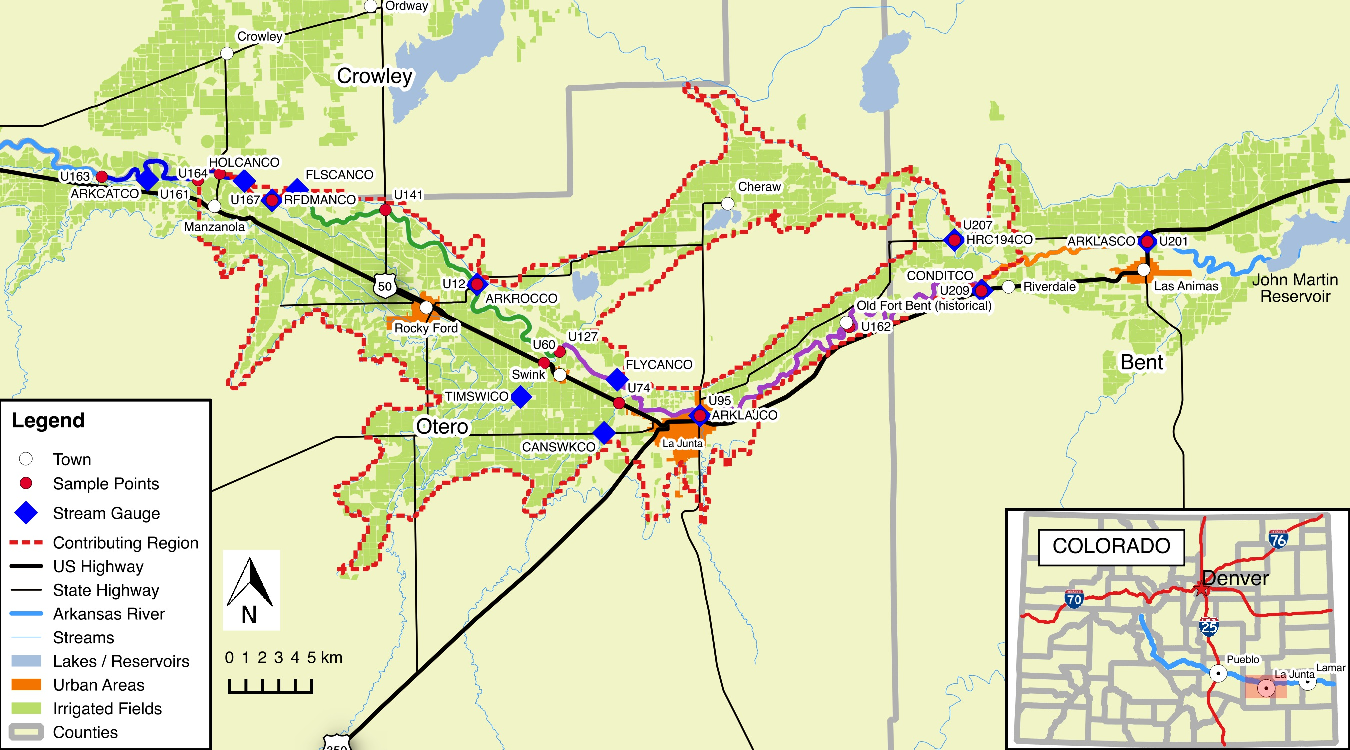
\includegraphics[scale=1]{Figures/Map/USRSample}
		\caption[Dissolved Se sampling locations in the USR.]{Dissolved Se sampling locations in the USR.  Samples taken near, but not at stream gauge locations where shown.}
		\label{map:USRSample}
	\end{figure}
	\end{landscape}	
}

% Map - DSR sample locations
\afterpage{%
\clearpage%
	\begin{landscape}
	\begin{figure}
		\centering
		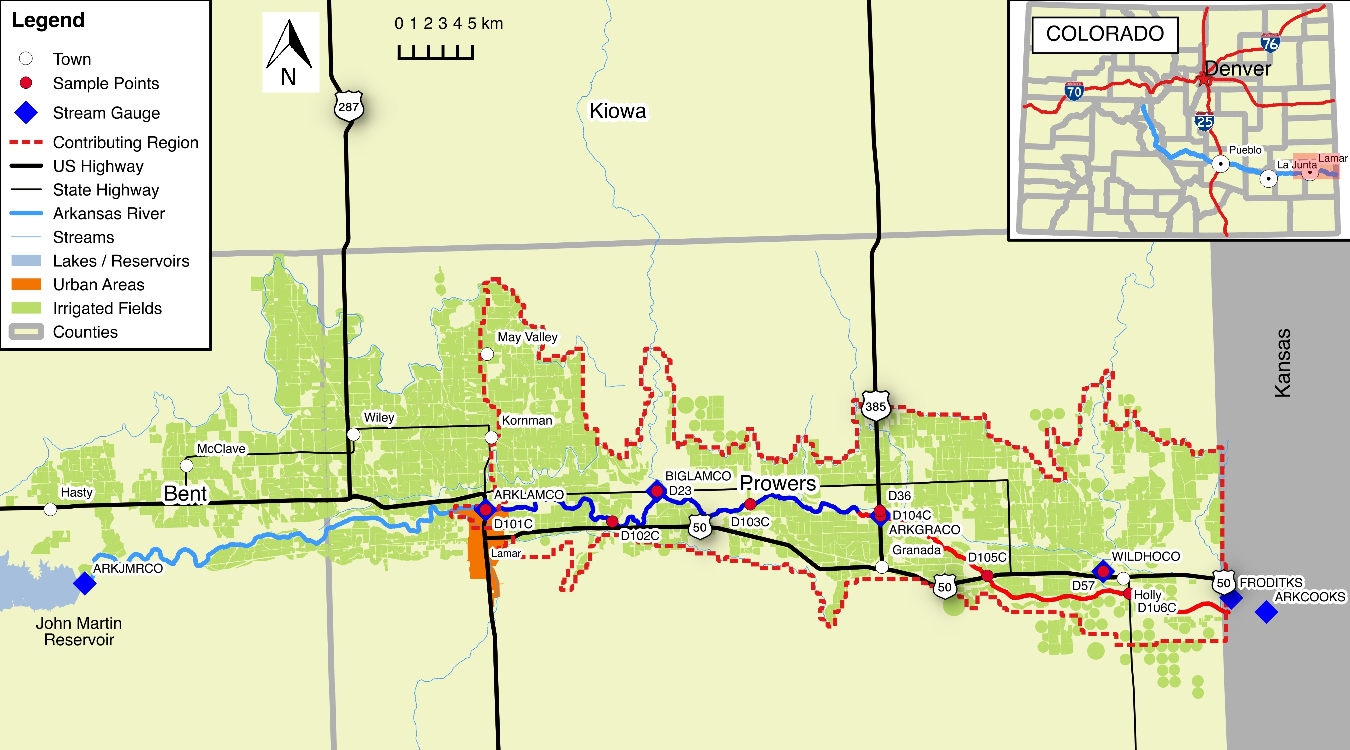
\includegraphics[scale=1]{Figures/Map/DSRSample}
		\caption[Dissolved Se sampling locations in the DSR.]{Dissolved Se sampling locations in the DSR.  Samples taken near, but not at stream gauge locations where shown.}
		\label{map:DSRSample}
	\end{figure}
	\end{landscape}	
}

% Table - USR sample locations
\begin{table}[htbp]
	\centering
	\caption[Upstream Study Region (USR) Sample Collection Point Information.]{Upstream Study Region (USR) Sample Collection Point Information.  A value of zero (0) indicates the location of the segment stream gauge.  Negative distances indicate the point is upstream of the reference stream gauge location. Segment B does not contain a stream gauge on the river main stem.}
	\label{tab:USRSampleLoc}
	\begin{tabular}{cccccc}
		\toprule
		River                       & Sample &  \multicolumn{2}{c}{Dist from}   &   \multicolumn{2}{c}{Dist from}   \\
		Segment                      & Point  & \multicolumn{2}{c}{USR Upstream} & \multicolumn{2}{c}{River Segment} \\
		Name                        &        &   \multicolumn{2}{c}{Boundary}   & \multicolumn{2}{c}{Stream Gauge}  \\
		\cmidrule(r{.5em}l){3-4} \cmidrule(r{.5em}l){5-6} &        &  mi  &            km             &  mi  &             km             \\ \toprule
		\multirow{3}{*}{A}                 &  U163  &  0   &             0             & -2.7 &            -4.3            \\
		&  U161  & 5.8  &            9.3            & 3.1  &             5              \\
		&  U164  & 6.8  &           10.9            & 4.1  &            6.6             \\ \midrule
		B                         &  U167  & 9.2  &           14.8            &      &  \\ \midrule
		\multirow{4}{*}{C}                 &  U141  & 14.7 &           23.7            & -5.5 &            -8.9            \\
		&  U12   & 20.2 &           32.5            &  0   &             0              \\
		&  U60   & 26.1 &            42             & 5.9  &            9.5             \\
		&  U127  & 26.4 &           42.5            & 6.2  &             10             \\ \midrule
		\multirow{4}{*}{D}                 &  U74   & 30.3 &           48.8            & -3.5 &            5.6             \\
		&  U95   & 33.8 &           54.4            &  0   &             0              \\
		&  U162  &  44  &           70.8            & 10.2 &            16.4            \\
		&  U209  & 52.8 &            85             &  19  &            30.6            \\ \midrule
		\multirow{2}{*}{E}                 &  U207  & 55.1 &           88.7            & -6.6 &           -10.6            \\
		&  U201  & 61.7 &           99.3            &  0   &             0              \\ \bottomrule
	\end{tabular}
\end{table}

% Table - DSR sample locations
\begin{table}[htbp]
	\centering
	\caption[Downstream Study Region (DSR) Se Sample Location Information.]{Downstream Study Region (DSR) Se Sample Location Information.  A value of zero (0) indicates the location of the segment stream gauge.  Negative distances indicate the point is upstream of the reference stream gauge location.}
	\label{tab:DSRSampleLoc}
	\begin{tabular}{cccccc}
		\toprule
		River                        & Sample &  \multicolumn{2}{c}{Dist from}   &   \multicolumn{2}{c}{Dist from}   \\
		Segment                       & Point  & \multicolumn{2}{c}{USR Upstream} & \multicolumn{2}{c}{River Segment} \\
		Name                         &        &   \multicolumn{2}{c}{Boundary}   & \multicolumn{2}{c}{Stream Gauge}  \\
		\cmidrule(r{0.5em}l){3-4} \cmidrule(r{0.5em}l){5-6} &        &  mi  &            km             &  mi  &             km             \\ \toprule
		\multirow{5}{*}{F}                  & D101C  &  0   &             0             &  0   &             0              \\
		& D102C  & 7.9  &           12.7            & 7.9  &            12.7            \\
		&  D23   & 11.6 &           18.7            & 11.6 &            18.7            \\
		& D103C  & 17.6 &           28.3            & 17.6 &            28.3            \\
		&  D36   & 23.4 &           37.7            & 23.4 &            37.7            \\ \midrule
		\multirow{4}{*}{G}                  & D104C  & 24.9 &           40.1            &  0   &             0              \\
		& D105C  & 31.2 &           50.2            & 6.3  &            10.1            \\
		&  D57   & 38.1 &           61.3            & 13.2 &            21.2            \\
		& D106C  & 38.9 &           62.6            &  14  &            22.5            \\ \bottomrule
	\end{tabular}
\end{table}

Sample collection trips involved hours of preparation.  Before leaving for the study region(s), equipment and supplies were prepared.  Peristaltic pumps were used for all surface water sample collection.  Two Durham Geo TR-200 PSP peristaltic pumps were taken on each trip.  The TR-200 is a single head, bi-directional, 12-volt battery operated, portable sampling pump capable of delivering flow rates up to \SI{500}{\milli\liter\per\minute} in both directions (Figure \ref{pic:pump}).  The pumps were cleaned, in-situ water quality instruments were calibrated, and sample collection bottles were prepared.  Peristaltic pumps were cleaned at the beginning and end of each sampling day and before sampling at each field sampling location.  Figure \ref{pic:SampleVehicle} is a picture of a typical vehicle setup with cleaning buckets, peristaltic pump, water quality sonde, and various other equipment items.  Cleaning consisted of the following listed procedure:% listed in table xx.

\begin{enumerate}
	\item At the beginning of every sampling day, four, 5-gallon (gal) buckets with lids were prepared as follows:
	\begin{enumerate}
		\item One bucket filled with approximately \SI{2.5}{\gallon} tap water and approximately \SI{20}{\milli\liter} of lab grade hydrochloric acid (HCl).
		\item One bucket filled with approximately \SI{2.5}{\gallon} tap water and approximately \SI{20}{\milli\liter} of LiquiNox\textregistered, a lab grade, phosphate and ammonia free, free rinsing detergent.
		\item Two buckets filled with approximately \SI{2.5}{\gallon} deionized water.
	\end{enumerate}
	\item The acid solution was run through the pump for two minutes.  This disinfected the pump tubing and prevented cross contamination.
	\item The detergent solution was run through the pump for two minutes.  This removed any remaining soil particles from the pump tubing.
	\item Water from the first of the deionized water buckets was run through the pump for two minutes followed water from by the second bucket of deionized water for another two minutes.  This rinsed all detergent from the pump tubing.
\end{enumerate}

\begin{figure}[htbp]
	\centering
	\subcaptionbox{Durham Geo TR-200 PSP Peristaltic Pump.\label{pic:pump}}{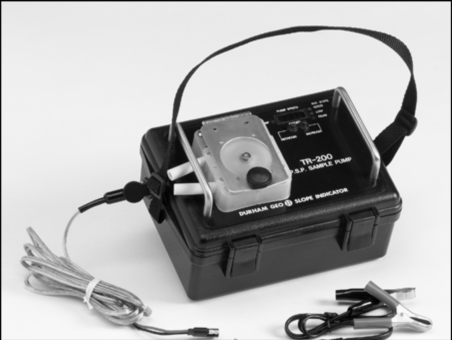
\includegraphics[width=2.5in]{Figures/Photo/PeristalticPump}}\hspace{4em}%
	\subcaptionbox{In Situ Water Quality Sonde and Data Logger.  Measures temperature, specific conductivity, pH, oxidation-reduction potential, and dissolved oxygen concentration.\label{pic:ysi}}{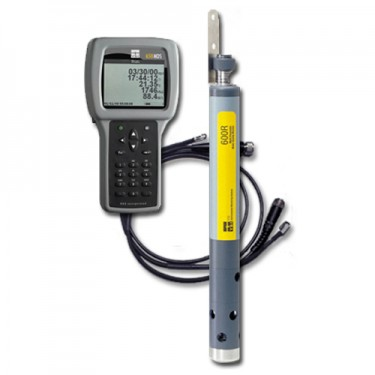
\includegraphics[width=2.5in]{Figures/Photo/ysi}}
	\caption[Water Quality Sampling Equipment.]{Water Quality Sampling Equipment.}
	\label{fig:WQEquipment}
\end{figure}

\begin{figure}
	\centering
	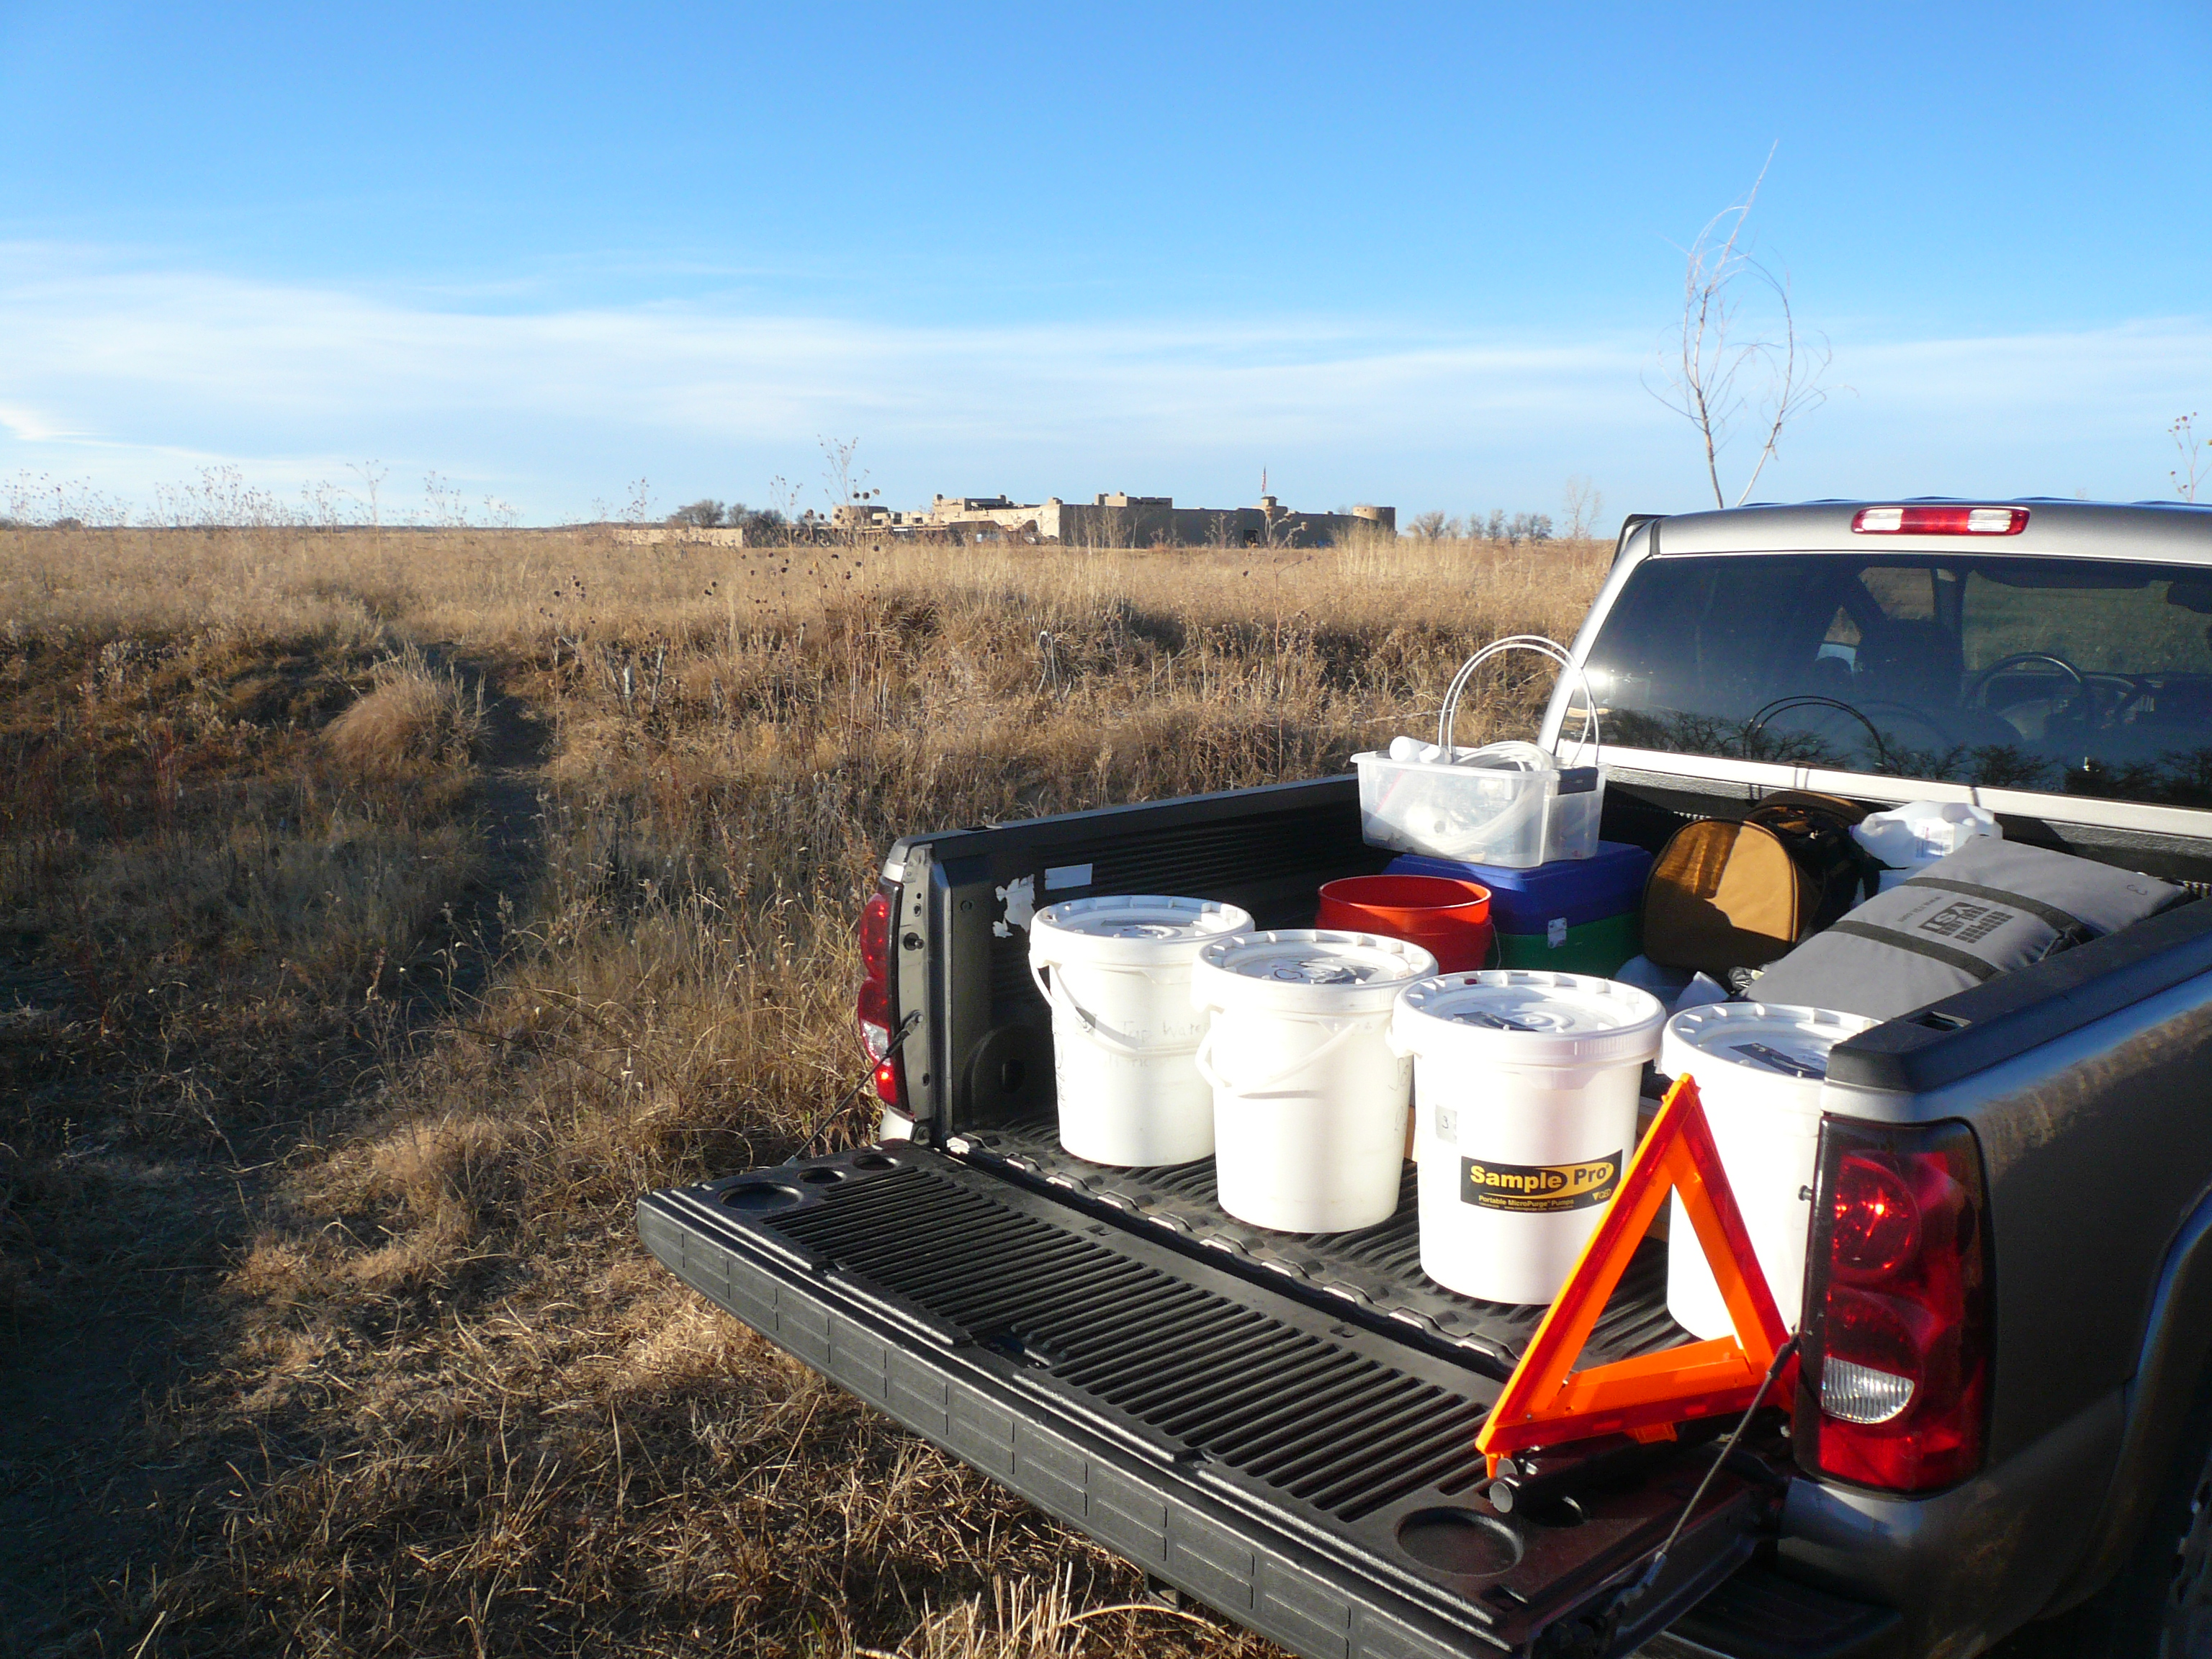
\includegraphics[width=4in]{Figures/Photo/SampleVehicle}
	\caption[Typical sample vehicle equipped for surface water sampling.]{Typical sample vehicle equipped for surface water sampling.  Equipment includes peristaltic pump, water quality sonde, pump cleaning buckets, and various other equipment items.  This picture is taken at sample site U162 which is on the National Park Service's Bent's Old Fort National Historic Site (fort in background).}
	\label{pic:SampleVehicle}
\end{figure}	

Two sample types were routinely taken at all locations during each trip.  One sample type was for the analysis of specific ion concentrations as a general water quality panel.  A \SI{250}{\milli\liter}-wide mouth, high density poly-ethylene (HDPE) bottle was used to collect and ship the specific ion samples.  This bottle was pre-cleaned and shipped to CSU by Ward Laboratories, Inc. in Kearney, Nebraska, the laboratory that provided the bulk of the water quality analysis services.  The second sample was taken for analysis of dissolved Se concentration using a \SI{125}{\milli\liter}-wide mouth, HDPE bottle.  This bottle was procured from multiple sources and pre-cleaned to the US EPA's "Specifications and Guidance for Contaminant Free Sample Containers" \parencite{EPA1992}.  Approximately \SI{0.6}{\milli\liter} of a diluted nitric acid solution prepared with \SI{33}{\milli\liter} of distilled water and \SI{7}{\milli\liter} of ultra-pure nitric acid was added to each bottle using a graduated pipette.  This was done to preserve the sample by lowering the pH to less than 2 standard pH units.  During the latter half of the sampling periods, samples for dissolved uranium (U) were gathered during most sampling trips.  \SI{250}{\milli\liter}-narrow mouth, pre-cleaned, pre-preserved with nitric acid, HDPE bottles were provided by TestAmerica Inc., the laboratory providing dissolved uranium analysis.

Blank samples of deionized water were prepared in the lab for each sample type before each trip at the beginning of each sampling day for each sample type.  Blanks are intended to be free of the analyzed constituent and are used to test the samples for bias due to contamination.  Trip blanks were taken in the lab before the begining of the sample trip.  They accompanied field personnel during all sampling activities and were then shipped to their respective lab for analysis.  Trip blanks were intended to demonstrate that there was no contamination due to transportation activities.  Field blanks were taken in the field at the begining of the sampling day.  These samples also accompanied the field personnel during sampling activities and were shipped to their respective lab for analysis.  Field blanks were intended to demonstrate that there was no contamination in the sampling equipment.   Any variation from non-detectable solute concentration in these blanks would indicate possible contamination of the water samples taken that day and further investigation would be required.  None of the lab results from field or trip blanks reported values that would indicate sample contamination.

Two YSI, Inc. 600R sondes with attached YSI, Inc. 650 MDS display data loggers were used for in-situ measurements during each sample trip (Figure \ref{pic:ysi}).  The sondes were equipped with a Rapid Pulse polarographic dissolved oxygen (DO) sensor capable of measuring DO from \SIrange{0}{50}{\milli\gram\per\liter}, \SI{\pm2}\%; a thermistor capable of measuring temperature from \SIrange{-5}{50}{\degreeCelsius}, \SI{\pm0.15}{\degreeCelsius}; a glass combination electrode pH sensor capable of measuring pH in the range of 0 to 14 units, $\pm$0.2 units; a platinum button oxidation-reduction potential (ORP) sensor capable of measuring in the range of \SIrange{-999}{999}{\milli\volt}, \SI{\pm20}{\milli\volt}; and a four electrode, autoranging  cell capable of measuring electrical conductivity (EC) as specific conductance at \SI{25}{\degreeCelsius} in the range of \SIrange{0}{100000}{\micro\siemens\per\centi\meter}, $\pm$0.5\%~+~\SI{1}{\micro\siemens\per\centi\meter}.  The equipment was serviced and calibrated by CSU field personnel before every trip to the study reaches and at the end of every sampling day.  Sondes were sent to Geotech Environmental Equipment, Inc. annually for maintenance checks.  Geotech Environmental Equipment, Inc. is an authorized dealer and service provider for YSI equipment with an office in Denver, Colorado.

At least one set of duplicate water samples was taken per sampling trip to the USR and/or DSR.  Duplicate, or replicate, samples were marked as 'A' and 'B' samples.  The 'A' sample results were kept with the main data set and were used as the primary data set.  'B' sample results were kept separate and were used to determine the combined sampling methodology and lab analysis uncertainty.  The sampling standard procedure was to take one duplicate set of surface water samples per day with a minimum of two duplicate surface water samples per sampling trip.

Each sampling event began with recording the site data on a form (log) similar to the one in Figure~\ref{fig:samplog}.  In-situ water quality measurements were then taken using the YSI sonde.  The data logger was used to read the data, but was not used as a recording device.  All data were recorded on the form shown as an example in Figure~\ref{fig:samplog}.  The ranges at the bottom of the form are maximum acceptable ranges of values determined from previous sampling trips.  Values outside of these ranges would indicate to field personnel that the equipment was damaged, had lost calibration, or operational error had occured.  The YSI sonde was allowed to rest in the water for a minimum of three minutes before recording values.  Usually, the sonde would rest in the water while water quality samples were taken.  Samples were pumped through a disposable, in-line \SI{0.45}{\micron}, polyethersulfone filter into the sample bottles.  Peristaltic pumps were used to extract all water samples from surface water sources.  No air space was permitted in any of the sample bottles.  Figure \ref{pic:samplingSub1} shows a trained sample collector at location U12 in the USR which is north of Rocky Ford on a bridge over the Arkansas River.  The YSI sonde is not in this image, but is suspended in the river during sample collection.  Figure \ref{pic:samplingSub2} is the same sample collector at sample location U73 in the USR recording readings from the YSI sonde.  Samples were stored on ice or in a refrigerator until they were shipped to their respective labs.  Data was recorded onto the data form from the YSI sonde immediately after collectiing the water samples.  The sonde was left in the water for an additional two to three minutes.  Any changes in readings were recorded as a second entry.  An example of a completed log is shown in Figure~\ref{fig:samplogComplete}

% Figure - blank sample log
\begin{figure}[htbp]
	\centering
	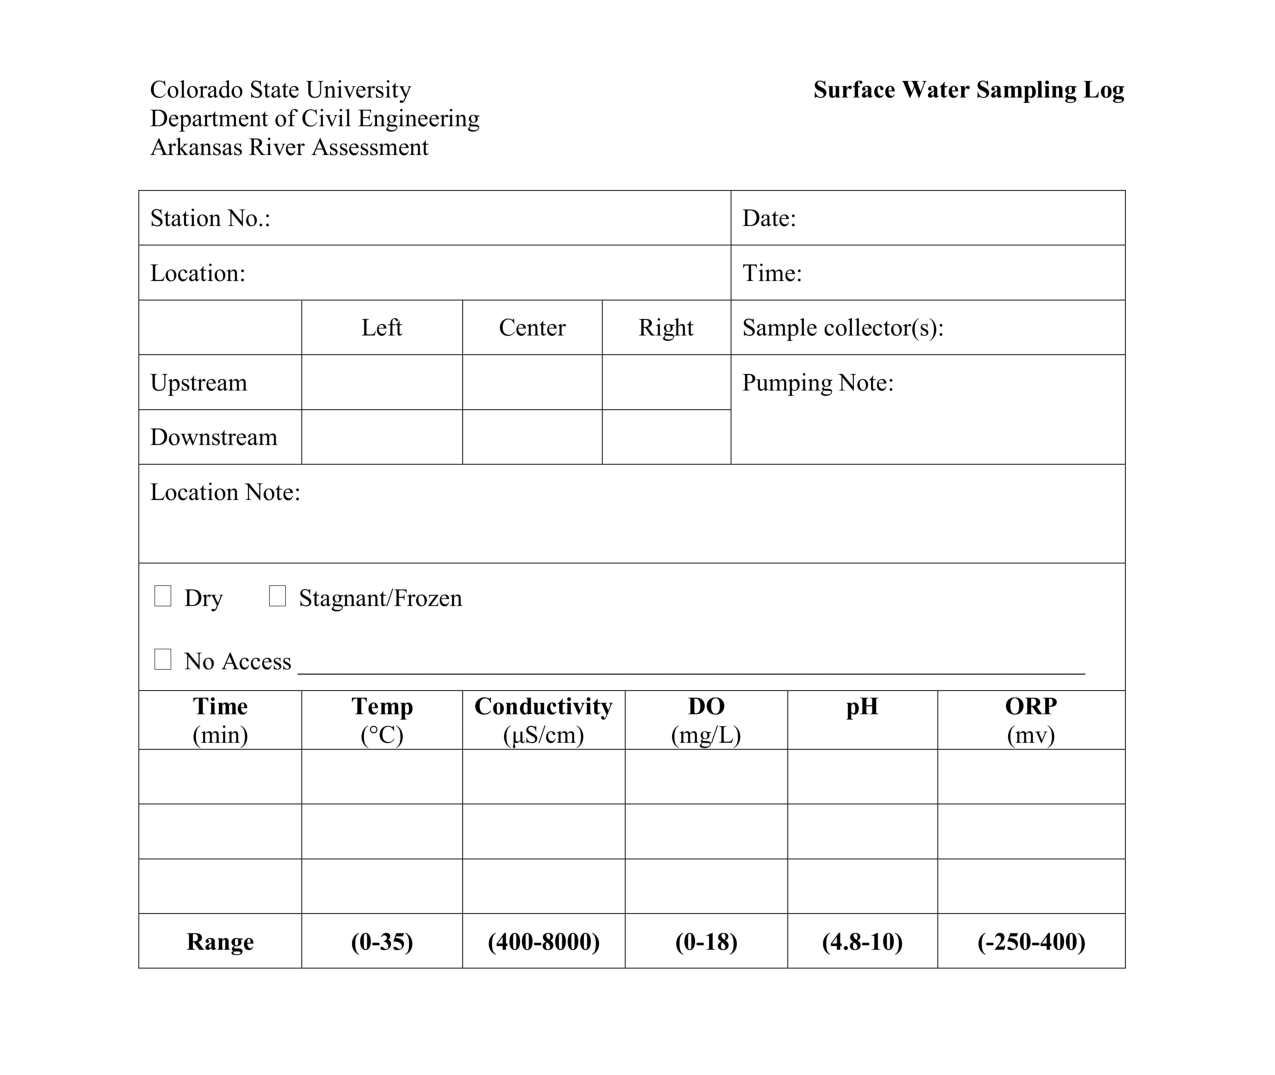
\includegraphics[width=6in]{Figures/SampleLog}
	\caption[Example water quality sample form.]{Example water quality sample form.}
	\label{fig:samplog}
\end{figure}

% Picture - samples being taken
\begin{figure}[htbp]
\centering
	\subcaptionbox{Sample location U12.  The Se sample bottle is being filled with a peristaltic pump through a \SI{0.45}{\micron} filter.  The specific ion sample bottle is filled, laying next to the pump.\label{pic:samplingSub1}}{\includegraphics[width=2.5in]{Figures/Photo/SampleFromBridge}}\hspace{4em}%
	\subcaptionbox{Sample location U73.   Personnel is hand logging data from the YSI sonde.\label{pic:samplingSub2}}{\includegraphics[width=2.5in]{Figures/Photo/SampleAtSmallTrib}}
	\caption[Personnel performing water sample collection.]{Personnel performing water sample collection.}
	\label{pic:sampling}
\end{figure}

% Figure - filled sample log
\begin{figure}[htbp]
	\centering
	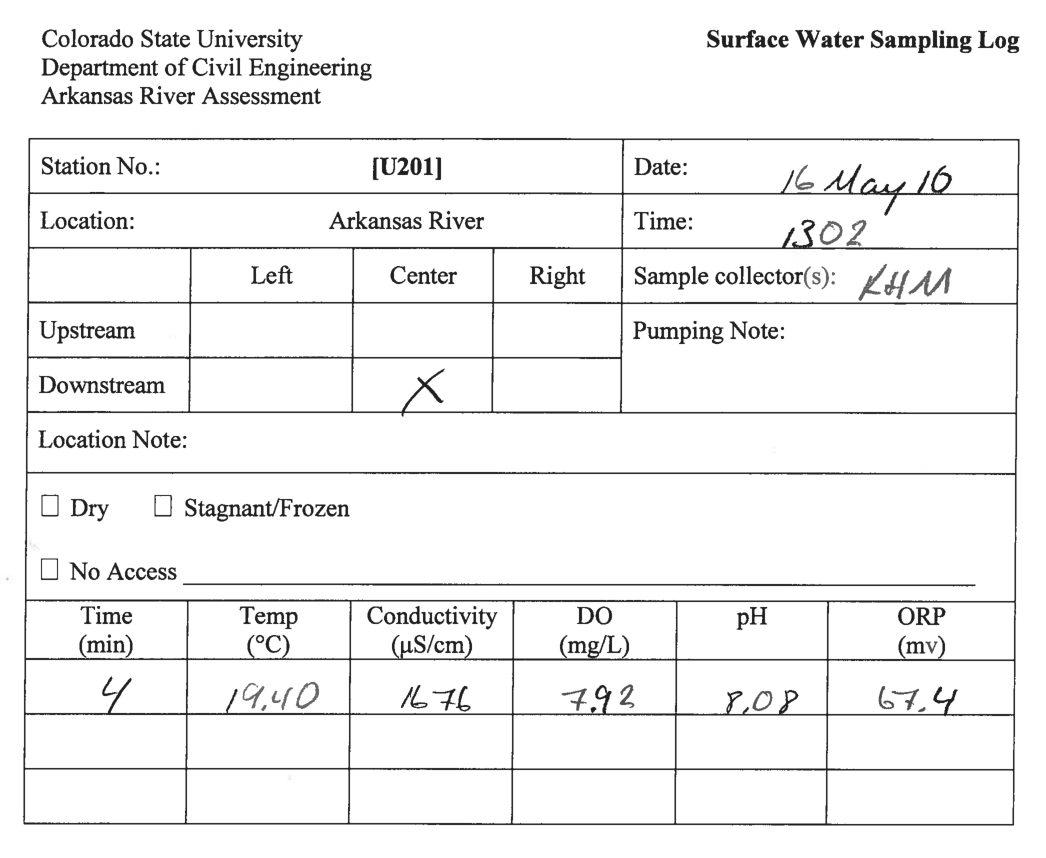
\includegraphics[width=6in]{Figures/SampleLogFilled}
	\caption[Example completed water quality sample form.]{Example completed water quality sample form.}
	\label{fig:samplogComplete}
\end{figure}

Specific ion lab results from Ward Laboratories and dissolved U lab results from TestAmerica were not used directly in the analysis reported in this tesis.  The Oscar E. Olson Biochemistry Laboratories (Olson Labs) at South Dakota State University (SDSU) performed dissolved Se analysis using Official Methods of Analysis of AOAC International, 17th Edition, test number 996.16, Selenium in Feeds and Premixes.  This test, a fluorometric test initially designed for testing animal feeds, provides repeatable analysis for dissolved Se near criteria levels.  Double tests were completed on each sample and the average was reported.  The minimum reportable value was \SI{0.4}{\micro\gram\per\liter}.  

Late in 2011, the Olson Labs was closed by SDSU for funding reasons.  Staff at Olson Labs assisted CSU staff in finding a new lab capable of continuing analyses using the same methods and to the same level of quality.  South Dakota Agricultural Laboratories (SDAL) was chosen.  Most of the staff and equipment from Olson Labs were employed at the new SDAL providing CSU staff with ample reason to move all dissolved Se analyses to the new lab.  Both Olson Labs and SDAL were certified by the USEPA for drinking water and subscribed to the proficiency testing and check sample programs for the USEPA for wastewaters \todo{ref.  How?}.

The same procedures and techniques for sample gathering and analysis were used during the entire sampling periods.  Newer or different techniques or procedures were considered, but was determined to have the possibility to compromise the consistency of the gathered data.  Results from all lab analyses were recorded in a master database at CSU for later data extraction and analysis.  The data includes results from over 4,500 sample sets.  Approximately 95 and 1,035 of these sample sets were taken from surface water sites in the USR and DSR, respectively.  Each sample set included in-situ measurements, a dissolved Se sample, a general specific ion panel, and a possible dissolved U sample.  In-situ EC and temperature measurements taken at stream gauge sites with permanent water quality instrumentation were compared with the measured values reported at those sites.  These sites record and report EC and water temperature measurements every 15-minutes.  Minor deviations were expected due to instrument drift and calibration error, yet EC and temperature differences were found to be less than 1\% for all in-situ measurements.

The water and mass balance models included in this study are among the many lines of research that have used this data.  Because of the multiple uses of large data sets, great care has been taken to ensure that data entry errors are rare.  Data were copied into the database and randomly checked for transcription errors.  Original lab reports were retained on file.

\clearpage{}
\section{River Cross-Section Geometry Survey}
The Arkansas River was surveyed at twenty-one and thirteen locations in the USR and DSR, respectively.  At these locations, cross-sections were surveyed and the data analyzed to determine the spatial distribution of the river geometry.  The cross-sections are not equally spaced along the river segments.  Cross-sections were surveyed at the extreme upstream and downstream end of each river segment.  Intermediate cross-sections were located where both the landowner permitted access and the river was reasonably accessible.  Additionally, the intermediate cross-sections were located where different cross-section profiles existed.  This was done to capture a broadest possible range of cross-section profiles, thereby allowing for a more realistic characterization of the river geometry.  Figures \ref{map:USRSurveyLocations} and \ref{map:DSRSurveyLocations} show the locations of the surveyed cross-sections in the USR and DSR, respectively.  Tables \ref{tab:USRSurveyLoc} and \ref{tab:DSRSurveyLoc} describe the location of the survey point with respect to the river reach and segment.  Survey locations within a river segment are with respect to the segment stream gauge location.

% Map - USR survey locations
\afterpage{%
	\clearpage%
	\begin{landscape}
	\begin{figure}[htbp]
		\centering
		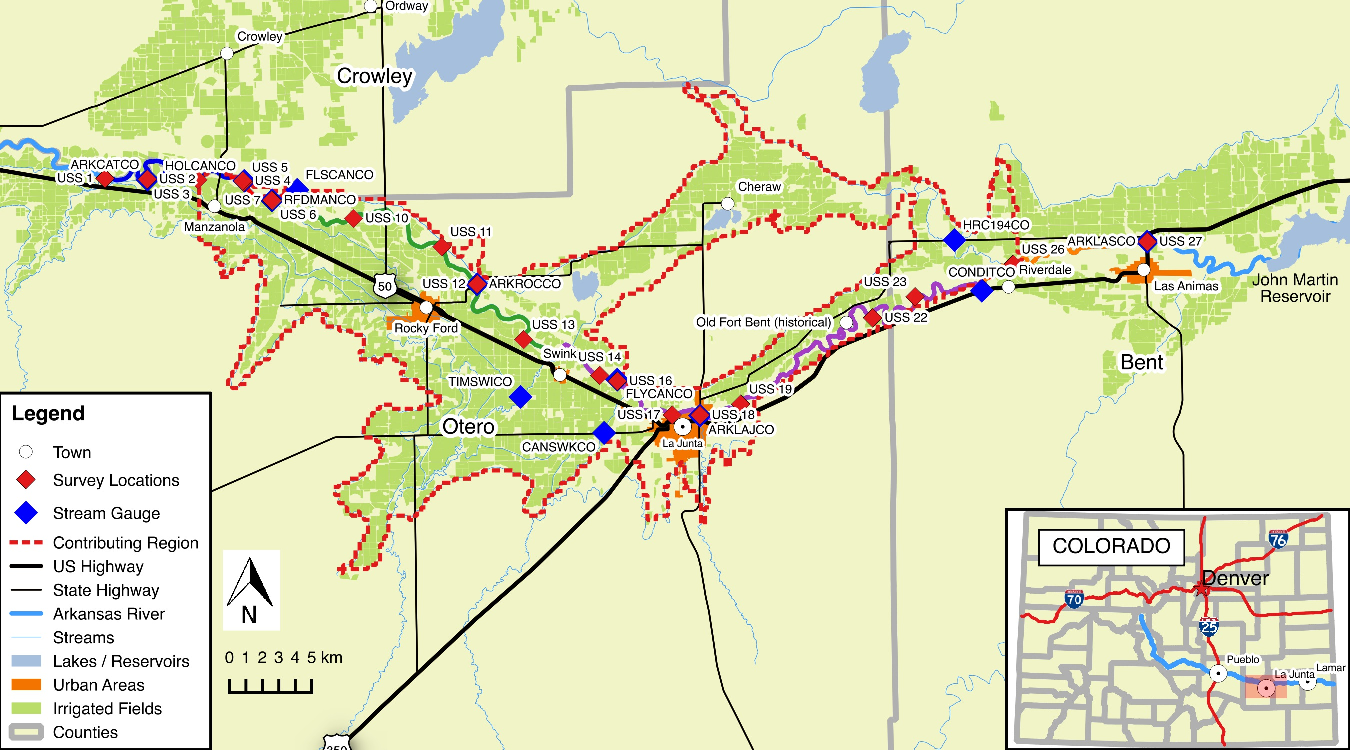
\includegraphics[scale=1]{Figures/Map/USRSurvey}
		\caption[USR River Cross-section Survey Locations.]{USR River Cross-section Survey Locations.  Cross-sections are taken above and/or below the diversion structure and near gauge locations.}
		\label{map:USRSurveyLocations}
	\end{figure}
	\end{landscape}
}

% Map - DSR survey locations
\afterpage{%
	\clearpage%
	\begin{landscape}
	\begin{figure}[htbp]
		\centering
		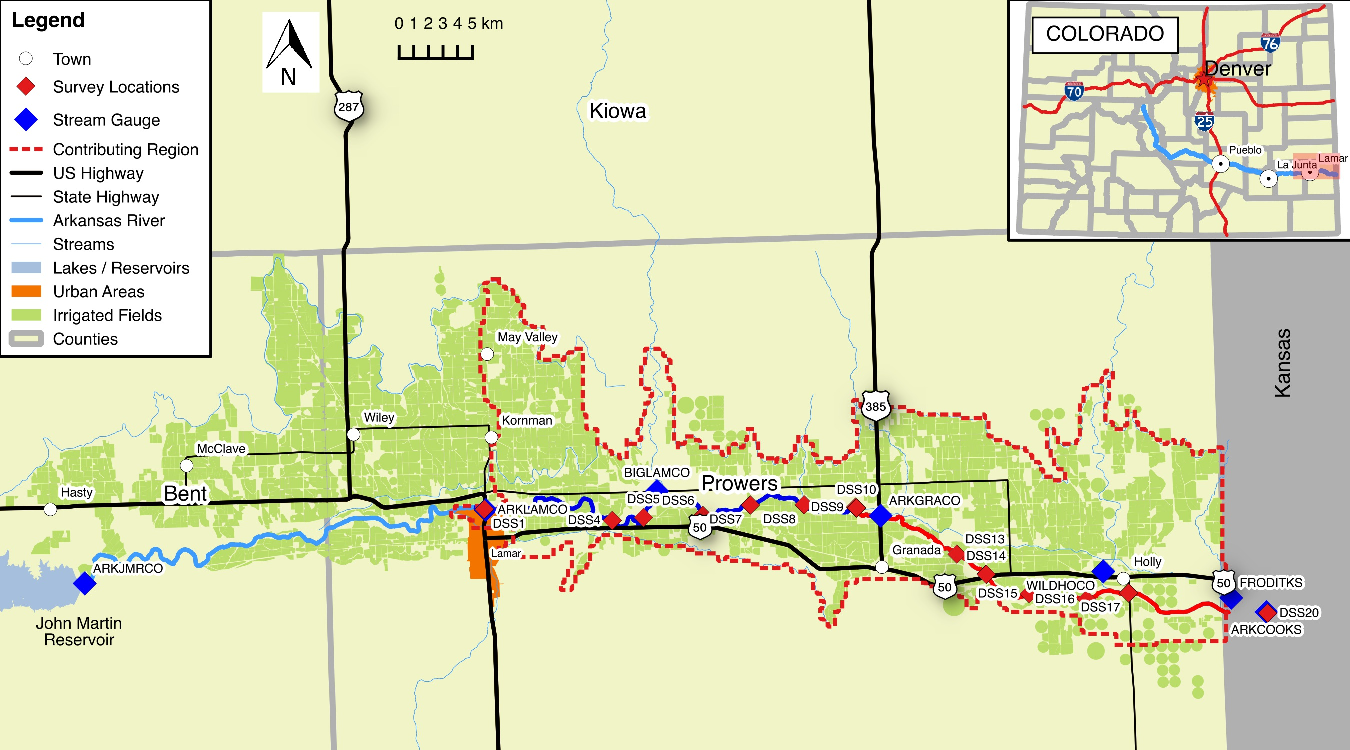
\includegraphics[scale=1]{Figures/Map/DSRSurvey}
		\caption[DSR River Cross-section Survey Locations.]{DSR River Cross-section Survey Locations.  Cross-sections are taken above and/or below the diversion structure and near gauge locations.}
		\label{map:DSRSurveyLocations}
	\end{figure}
	\end{landscape}
}

% Table - USR survey locations
\begin{table}[htbp]
	\centering
	\caption[Upstream Study Region (USR) Survey Point Information.]{Upstream Study Region (USR) Survey Point Information.  A value of zero (0) indicates the location of the segment stream gauge.  Negative distances indicate the point is upstream of the reference stream gauge location. Segment B does not contain a stream gauge on the river main stem.}
	\label{tab:USRSurveyLoc}
	\begin{tabular}{cccccc}
		\toprule
		River                       & Survey &  \multicolumn{2}{c}{Dist from}   &   \multicolumn{2}{c}{Dist from}   \\
		Segment                      & Point  & \multicolumn{2}{c}{USR Upstream} & \multicolumn{2}{c}{River Segment} \\
		Name                        &        &   \multicolumn{2}{c}{Boundary}   & \multicolumn{2}{c}{Stream Gauge}  \\
		\cmidrule(r{.5em}l){3-4} \cmidrule(r{.5em}l){5-6} &        &  mi  &            km             &  mi  &             km             \\ \toprule
		\multirow{4}{*}{A}                 &  USS1  &  0   &             0             & -2.7 &            -4.3            \\
		&  USS2  & 2.7  &            4.3            &  0   &             0              \\
		&  USS3  & 5.8  &            9.3            & 3.1  &             5              \\
		&  USS4  & 7.8  &           12.6            & 5.1  &            8.2             \\ \midrule
		\multirow{3}{*}{B}                 &  USS6  & 9.2  &           14.8            &      &  \\
		&  USS7  & 9.3  &           14.9            &      &  \\
		&  USS8  & 10.2 &           16.4            &      &  \\ \midrule
		\multirow{5}{*}{C}                 & USS10  & 13.4 &           21.6            & -6.8 &           -10.9            \\
		& USS11  & 18.1 &           29.1            & -2.1 &            -3.4            \\
		& USS12  & 20.2 &           32.5            &  0   &             0              \\
		& USS13  & 24.4 &           39.3            & 4.2  &            6.8             \\
		& USS14  & 29.3 &           47.2            & 9.1  &            14.6            \\ \midrule
		\multirow{7}{*}{D}                 & USS16  &  30  &           48.3            & -3.8 &            -6.1            \\
		& USS17  & 32.6 &           52.5            & -1.2 &            -1.9            \\
		& USS18  & 33.8 &           54.4            &  0   &             0              \\
		& USS19  & 35.9 &           57.8            & 2.1  &            3.4             \\
		& USS21  &  44  &           70.8            & 10.2 &            16.4            \\
		& USS22  & 46.4 &           74.7            & 12.6 &            20.3            \\
		& USS23  & 50.3 &            81             & 16.5 &            26.6            \\ \midrule
		\multirow{2}{*}{E}                 & USS26  & 55.7 &           89.6            &  -6  &            -9.7            \\
		& USS27  & 61.7 &           99.3            &  0   &             0              \\ \bottomrule
	\end{tabular}
\end{table}

% Table - DSR survey locations
\begin{table}[htbp]
	\centering
	\caption[Downstream Study Region (DSR) River Cross-Section Survey Location Information.]{Downstream Study Region (DSR) River Cross-Section Survey Location Information.  A value of zero (0) indicates the location of the segment stream gauge.  Negative distances indicate the point is upstream of the reference stream gauge location.}
	\label{tab:DSRSurveyLoc}
	\begin{tabular}{cccccc}
		\toprule
		River                        & Survey &  \multicolumn{2}{c}{Dist from}   &   \multicolumn{2}{c}{Dist from}   \\
		Segment                       & Point  & \multicolumn{2}{c}{USR Upstream} & \multicolumn{2}{c}{River Segment} \\
		Name                         &        &   \multicolumn{2}{c}{Boundary}   & \multicolumn{2}{c}{Stream Gauge}  \\
		\cmidrule(r{0.5em}l){3-4} \cmidrule(r{0.5em}l){5-6} &        &  mi  &            km             &  mi  &             km             \\ \toprule
		\multirow{7}{*}{F}                  &  DSS1  &  0   &             0             &  0   &             0              \\
		&  DSS4  & 7.9  &           12.7            & 7.9  &            12.7            \\
		&  DSS5  & 10.3 &           16.6            & 10.3 &            16.6            \\
		&  DSS6  & 14.9 &            24             & 14.9 &             24             \\
		&  DSS7  & 17.6 &           28.3            & 17.6 &            28.3            \\
		&  DSS8  & 20.5 &            33             & 20.5 &             33             \\
		&  DSS9  & 23.4 &           37.7            & 23.4 &            37.7            \\ \midrule
		\multirow{6}{*}{G}                  & DSS10  & 23.5 &           37.8            & -1.4 &            -2.3            \\
		& DSS13  & 29.3 &           47.2            & 4.4  &            7.1             \\
		& DSS14  & 31.2 &           50.2            & 6.3  &            10.1            \\
		& DSS15  & 33.9 &           54.6            &  9   &            14.5            \\
		& DSS16  &  37  &           59.5            & 12.1 &            19.5            \\
		& DSS17  & 38.9 &           62.6            &  14  &            22.5            \\ \midrule
		& DSS20  & 46.2 &           74.4            &      &  \\ \bottomrule
	\end{tabular}
\end{table}

Industry standard survey techniques were used whenever possible.  It was not possible to properly locate the instrument location in either the horizontal and vertical plane with respect to a local datum due to the remote location and the lack of available time.  All data was collected with a total station (Figure \ref{pic:surveySub1})and hand recorded into survey log books.  Two back-sights were used at every surveyed cross-section.  Both back-sights and the instrument location were located by using a hand held global positioning satellite (GPS) receiver (Figure \ref{pic:surveySub2}).  The receiver was capable of determining the horizontal location to within \SI{\pm 1}{\meter} and the vertical location to within \SI{\pm 2}{\meter}.  Licensed surveyors were not hired, retained, or consulted for this study.

% Picture - total station and GPS
\begin{figure}[htbp]
	\subcaptionbox{Pentax PCS-315 Total Station.\label{pic:surveySub1}}{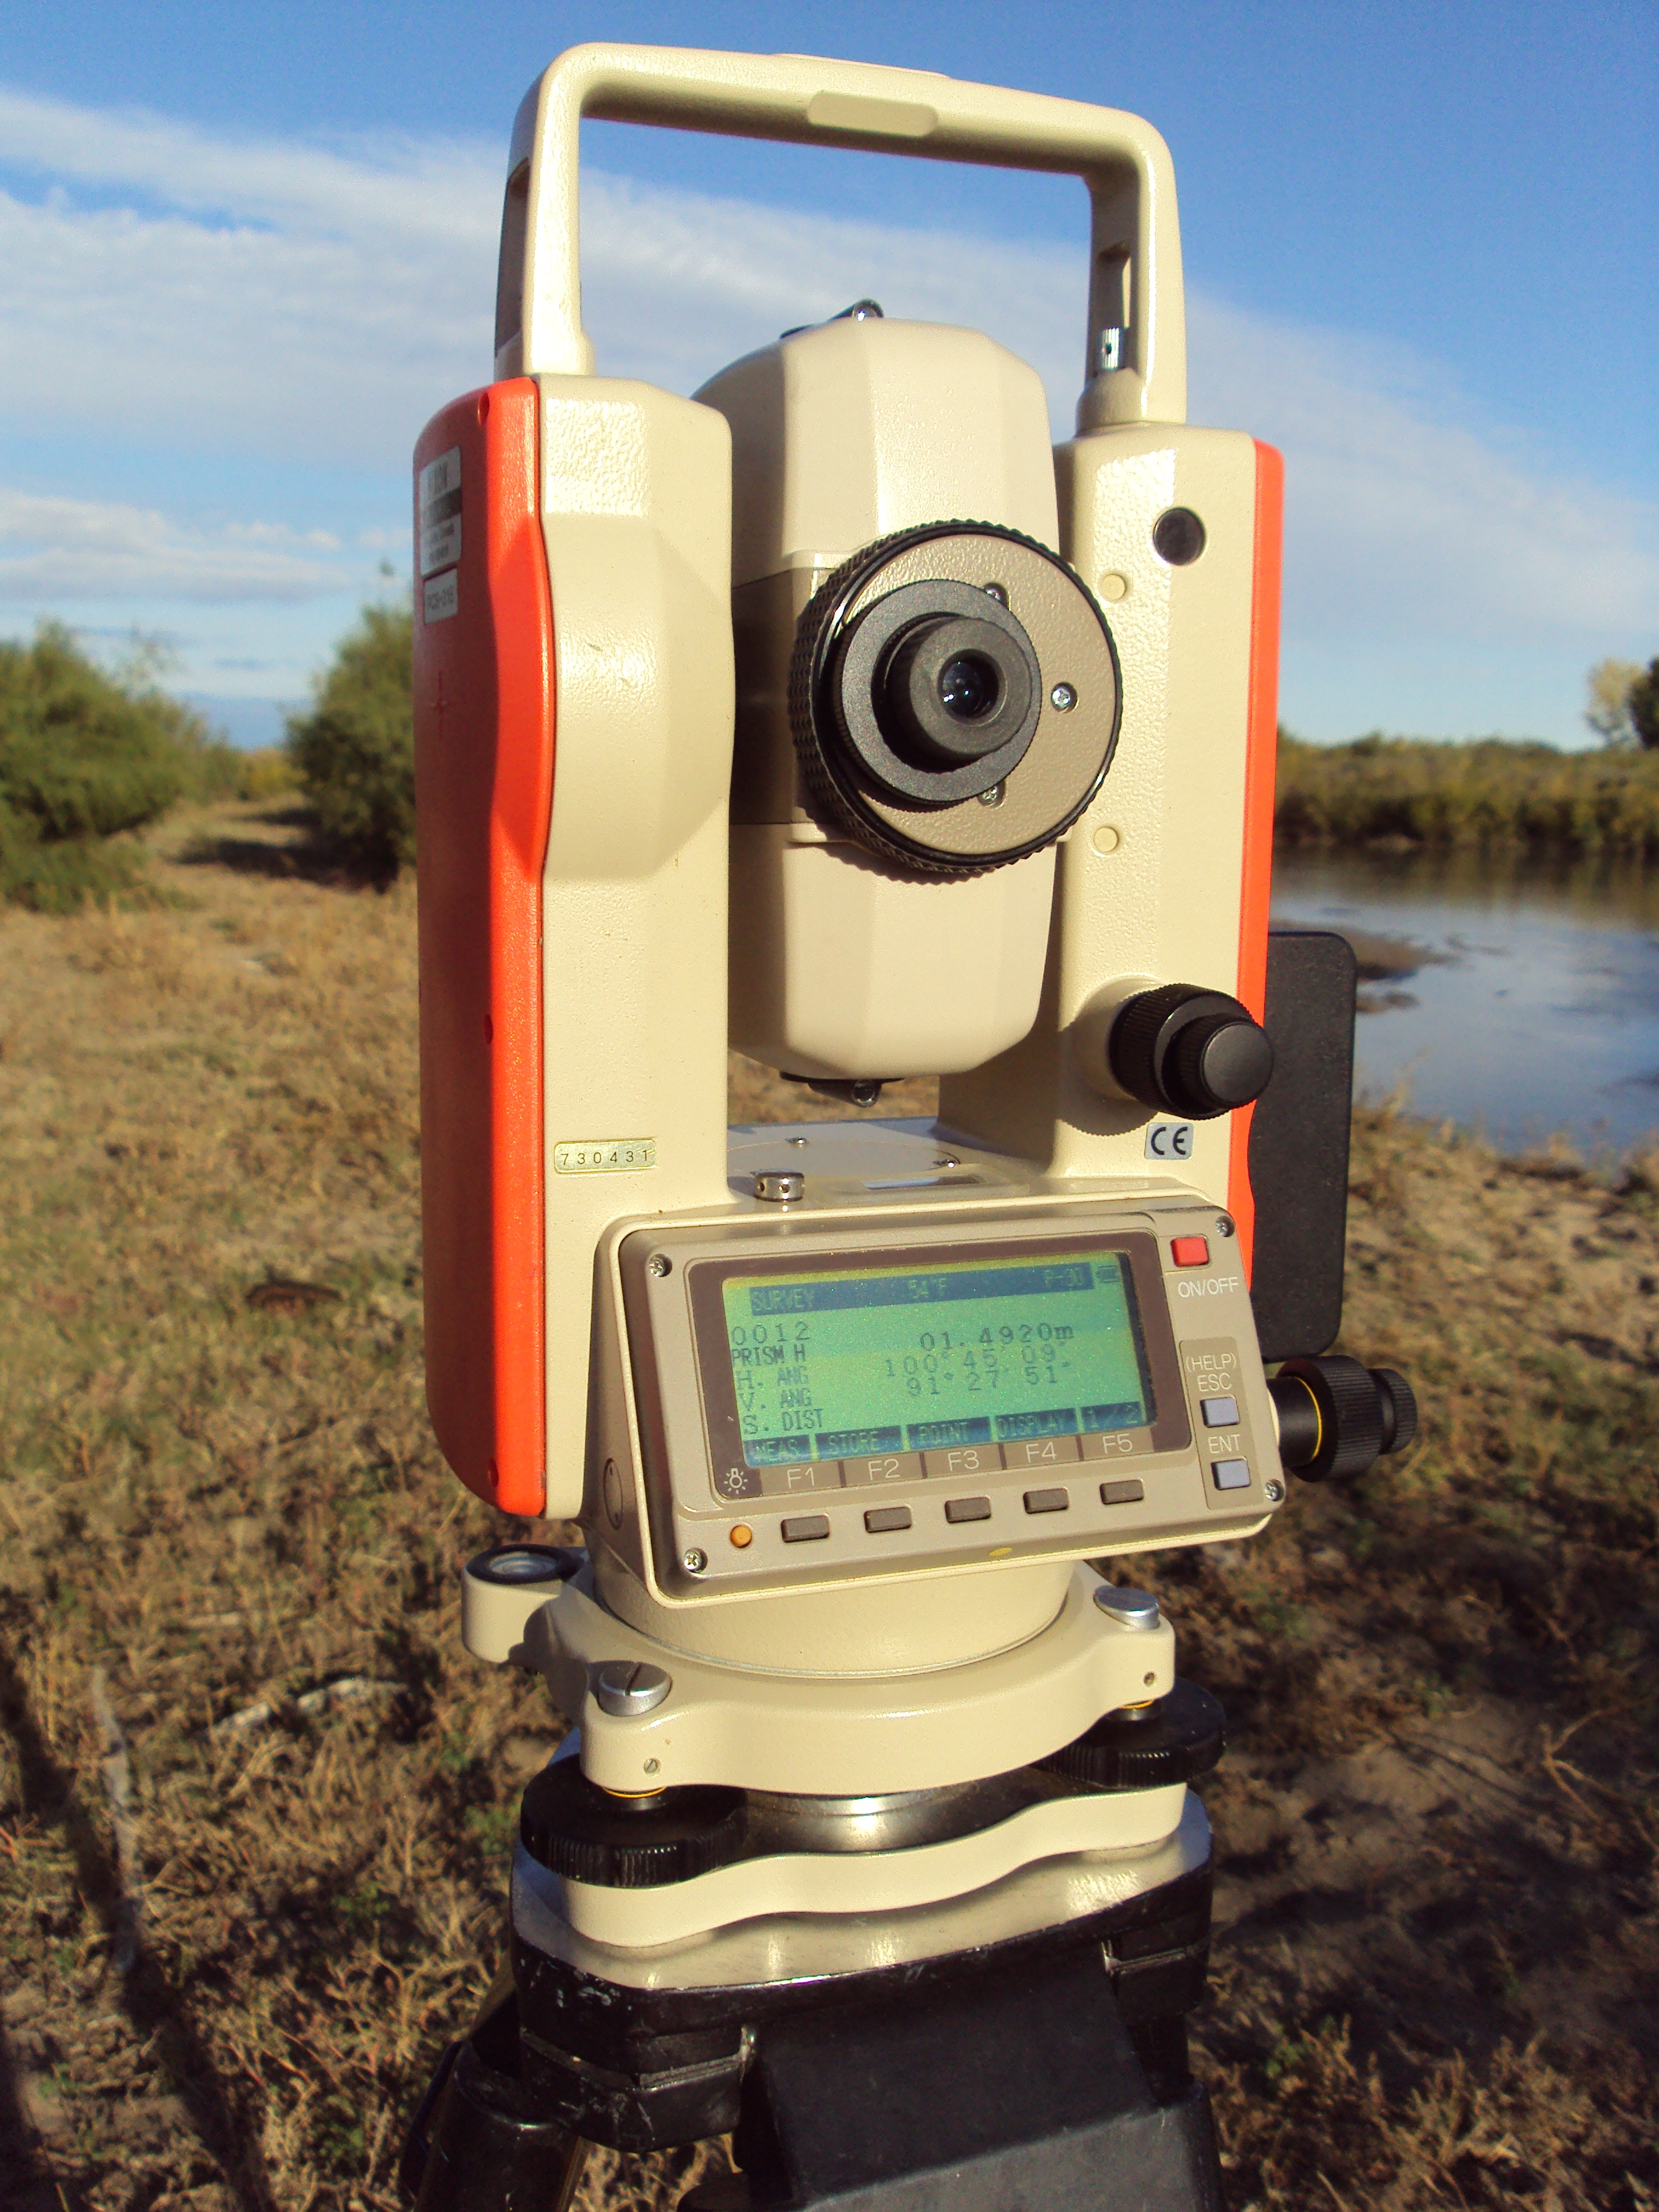
\includegraphics[width=2.5in]{Figures/Photo/TotalStation}}\hspace{4em}%
	\subcaptionbox{TopCon GMS-2 Sub-meter handheld GPS.\label{pic:surveySub2}}{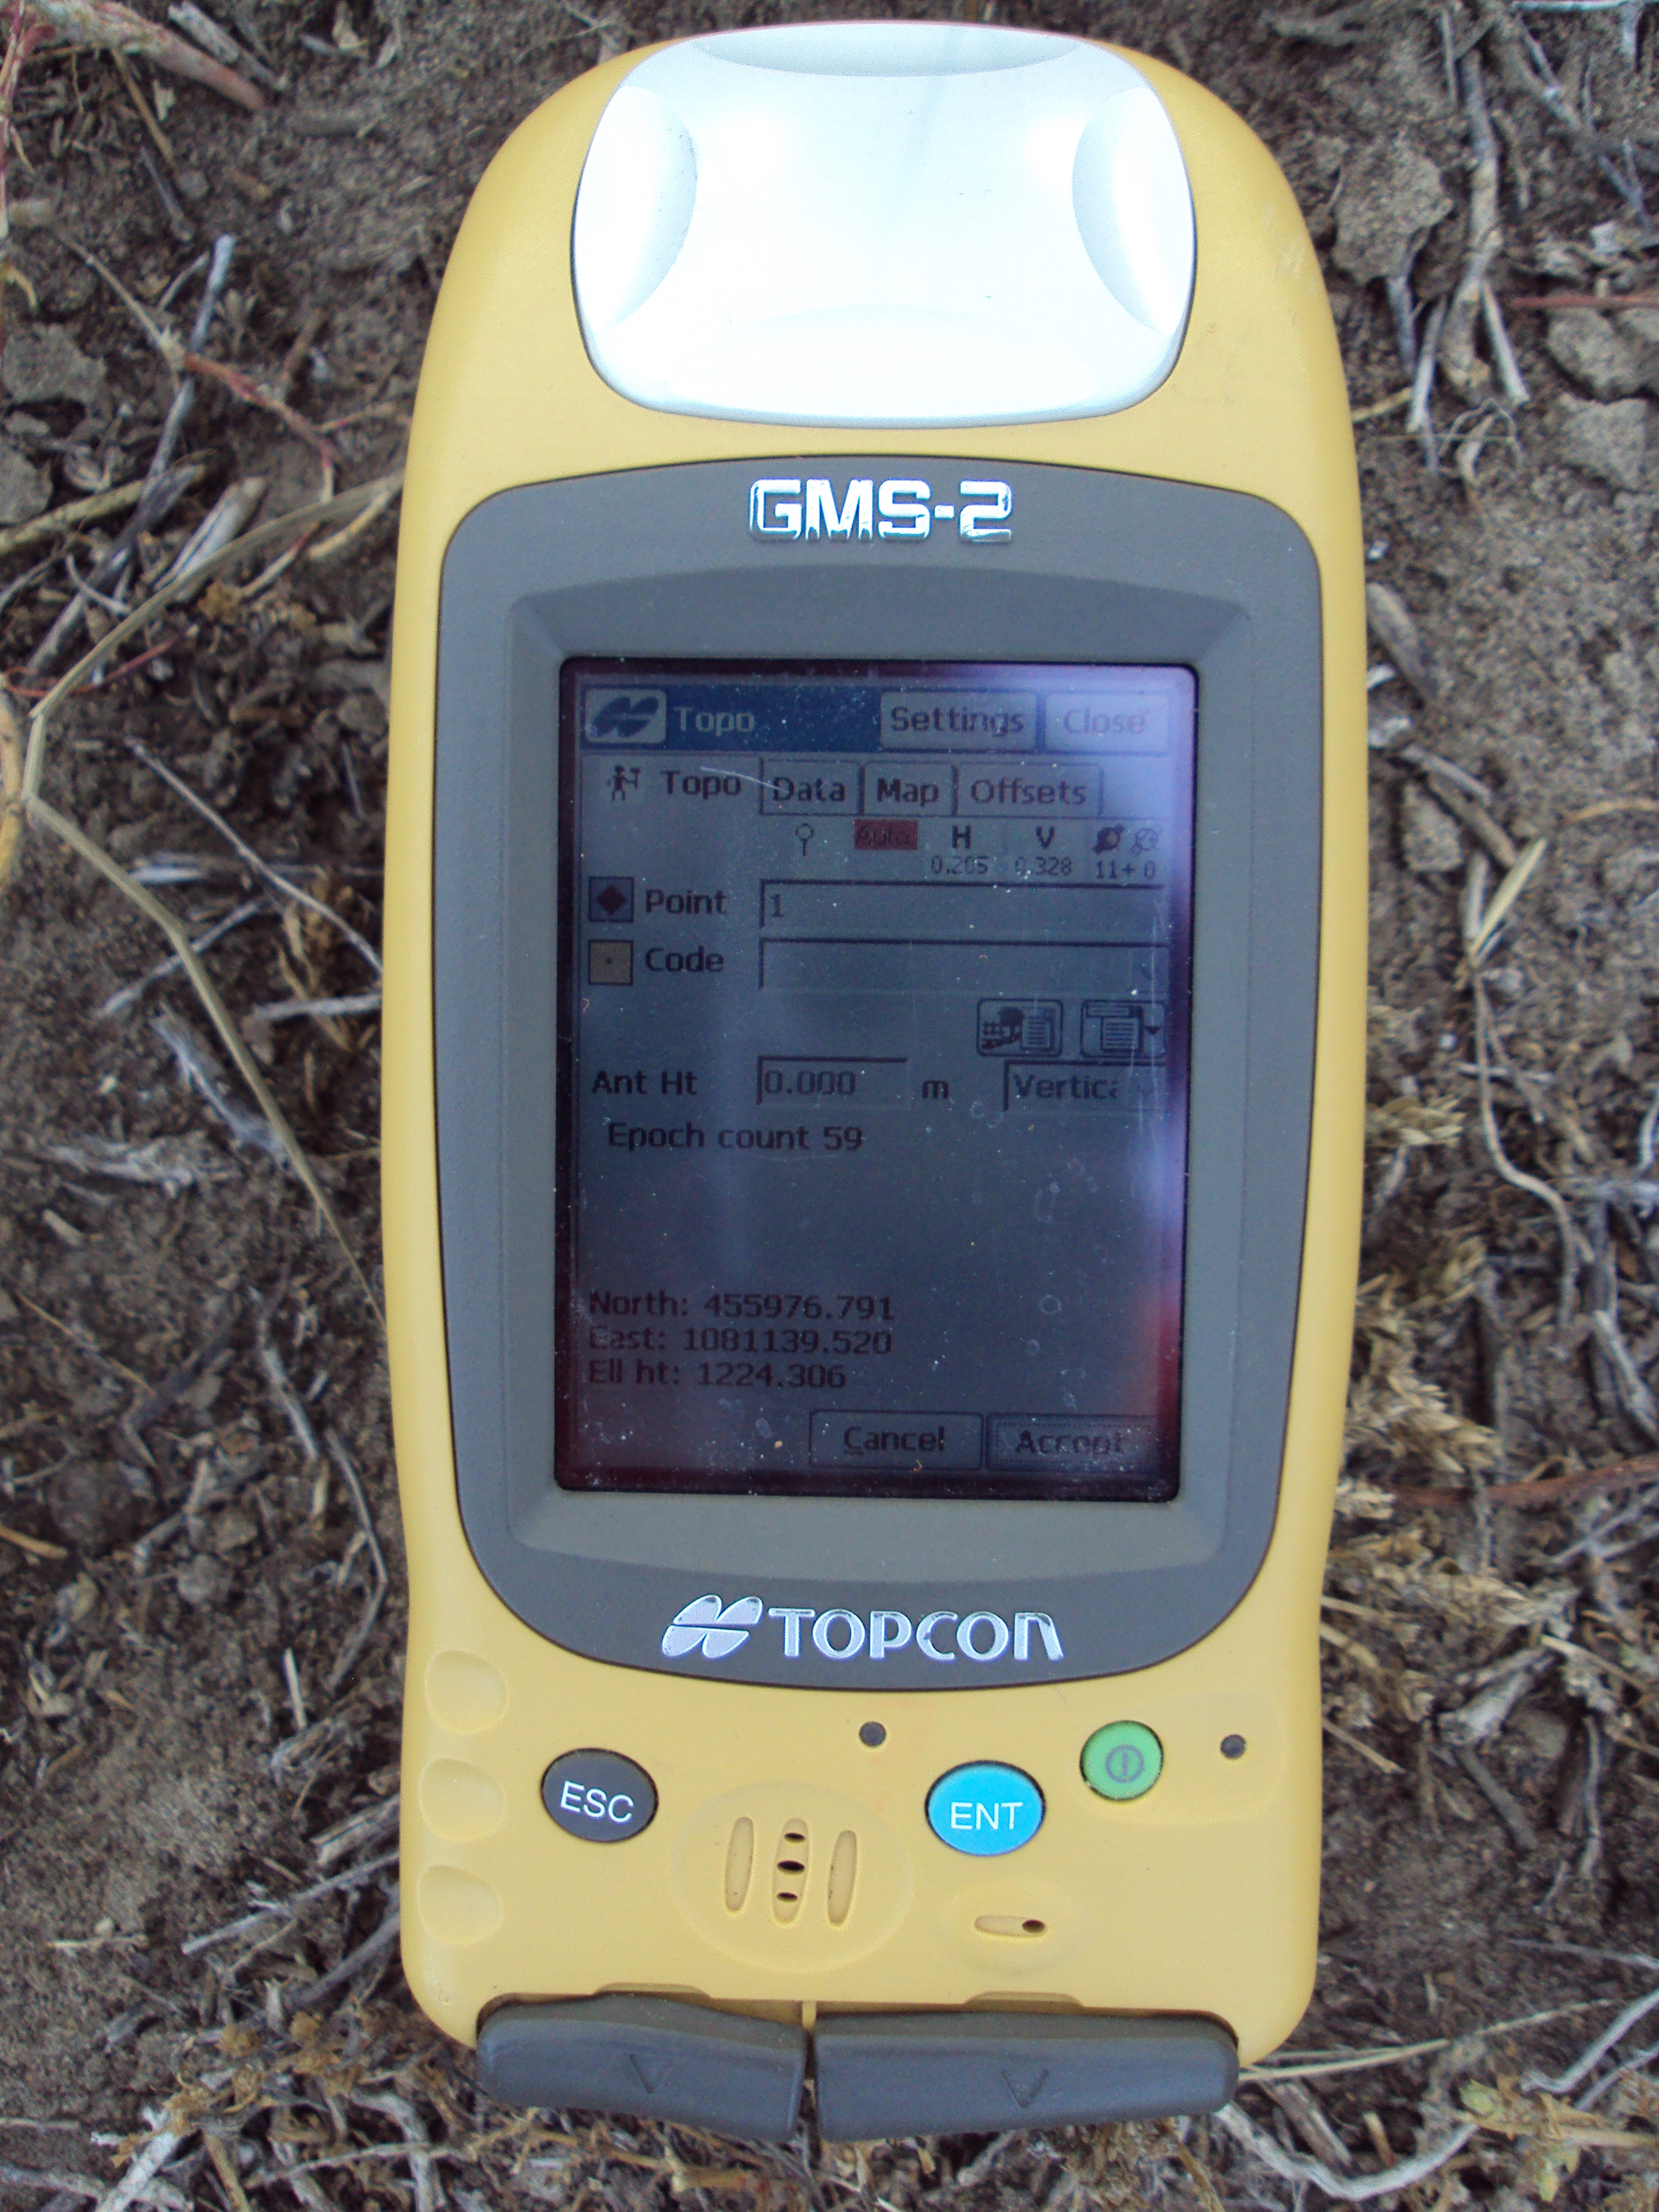
\includegraphics[width=2.5in]{Figures/Photo/SubMeterGPS2}}
	\caption[Survey Equipment.]{Survey Equipment.}
	\label{pic:surveyEquip}
\end{figure}

Higher location and orientation accuracy could have been obtained by using survey grade GPS equipment or by referencing the instrument survey to an established benchmark.  For almost all surveyed cross-sections, benchmarks were not located within a reasonable distance.  Attempting to tie into these benchmarks would results in an order of magnitue or more increase in the time required to complete the survey.  There were also doubts as to whether the horizontal and vertical accuracy could be maintained due to the distance between the nearest benchmarks and the survey sites and the surveyor's skill.  Survey grade GPS equipment could have been used, but would have required either a larger team or a significantly increased risk of equipment tampering or theft.  The available survey grade GPS base station also had a limited range compared to the range required to access many of the locations.  Since the goal of the survey was to determine the relationship between the depth and width of the river, it was determined that locating and orienting the survey data correctly was a secondary goal. For these reasons, it was determined that the level of location and orientation accuracy obtained by using the hand held GPS receiver would be sufficient.

The data was collected in the form of horizontal angle, vertical angle, sight distance, rod height, and instrument height.  The survey data was downloaded from the total station and entered into a spreadsheet for conversion to horizontal and vertical location relative to the instrument.  Values in the spreadsheet were checked against the survey log book.  Points collected but not used to calculate the cross-section, such as the back-sight points, were marked so that they were not used in the cross-section analysis.  These excluded points were used for other survey related calculations.  The rod height for each measurement and the instrument height for the survey was transferred from the log book to the spreadsheet.  

Coordinate geometry (COGO) techniques were used to convert from angle, sight distance, rod height, and instrument height measurements to horizontal and vertical distance measurements relative to the instrument as shown in figure \ref{fig:SurveyMeasurements}.  Vertical angles were measured using decimal degrees such that zero degrees (\SI{0}{\degree}) was located above the instrument and \SI{90}{\degree} was horizontal.  Horizontal angles were measured using decimal degrees such that \SI{0}{\degree} was located when the instrument was facing the first back-sight and positive angles were measured clockwise when viewed from above.  The sight distance was measured using the instruments integrated laser distance measuring tool from the optics of the instrument to the rod prism with sub-millimeter accuracy.  Horizontal and vertical distances to the ground location of the survey point from the ground location of the instrument were calculated as shown in equations \ref{eq:horizontal} and \ref{eq:vertical}, respectively.  The horizontal location was calculated as northing and easting with the line between the instrument and the first back-sight as the reference.  Northing and easting distances were calculated with respect to the horizontal line between the instrument and the first backsight.  Corrections were made to orient the points to the coordinate system, but this step was not necessary to provide the necessary results. %as shown in equations \ref{eq:northing} and \ref{eq:easting}, respectively.

% Figure - Survey measurements.  Includes equation.
\begin{figure}[htbp]
	\centering
	\includegraphics[scale=1]{Figures/LineDiagram/SurveyMeasurements}

\begin{align}
	d_h=&\:d_s \cdot sin(\theta_v) \label{eq:horizontal} \\
	\nonumber \\
	d_v=&\:h_i-h_r+d_s \cdot cos(\theta_v) \label{eq:vertical}
\end{align}
%	d_N=&d_h \cdot cos(\theta_h) \label{eq:northing} \\  %% took out the horizontal measurements.  Not particularly relevant.
%	d_E=&d_h \cdot sin(\theta_h) \label{eq:easting}
\begin{tabular}{r l}
	        $d_h$ = & Horizontal distance from the instrument to the surveyed point.                    \\
	        $d_v$ = & Vertical distance from the instrument to the surveyed point.                      \\
	      %	$d_N$ = & Horizontal distance from the instrument to the surveyed point as projected on the \\
	              % & East-West line passing through the instrument (northing).                         \\
	              % &  \\
	      %	$d_E$ = & Horizontal distance from the instrument to the surveyed point as projected on the \\
	              % & North-South line passing through the instrument (easting).                        \\
	              % &  \\
	        $d_s$ = & Sight distance from the instrument optics to the rod prism.                       \\
	   $\theta_v$ = & Vertical angle from the sight optics to the rod prism                             \\
	%	$\theta_h $ = & Horizontal angle from the sight optics to the rod prism                           \\
	              % &
\end{tabular}
	\caption[Survey Measurement Definitions.]{Survey Measurement Definitions.}
	\label{fig:SurveyMeasurements}
\end{figure}

GPS location data for the instrument and back-sights was collected in the form of northing, easting, and elevation.  Colorado State Plane-South, North American Datum 1983 (NAD83), U.S. feet was used as the horizontal datum and North American Vertical Datum 1988 (NAVD88) was used as the vertical datum.  All survey units are U.S. Feet.  Survey errors, also known as closing errors, were corrected for all points.  Most survey locations were on soft soils.  It was assumed that survey error would primarily consist of instrument location drift.  Measurements were taken to both back-sights at the beginning an end of the site survey.  The northing, easting, and elevation difference between the measurements taken at the beginning and end of the site survey were spread equally and successively among all points.  Since two back-sights were used, the total closing error was taken as the average of the closing errors for the two back-sights.  

Correction of closing errors was required to obtain accurate stream depth and river top width values.  Location and orientation error correction was not required and was only performed as a manner of good survey practice.  Survey data points were translated from their position relative to the instrument to their position relative to the State Plane coordinate system by adding the northing, easting, and elevation values collected by the GPS receiver at the instrument site.  Orientation error corrections to make instrument North coincide with true North were made by adding a positive horizontal correction angle such that the corrected angle to the first back-sight, which was the zero back-sight, matched the angle between the two corresponding GPS northing and easting coordinate sets.  Final survey locations should always have the most correct location and elevation relative to a given datum.  Both the back-sights and instrument location were marked with steel reinforcement bar (re-bar) and plastic caps (Figure \ref{pic:plasticCap}), it may be possible for future surveys to be conducted at the same locations with the same back-sights.

% Picture - control point/plastic cap
\begin{figure}[htbp]
\centering
	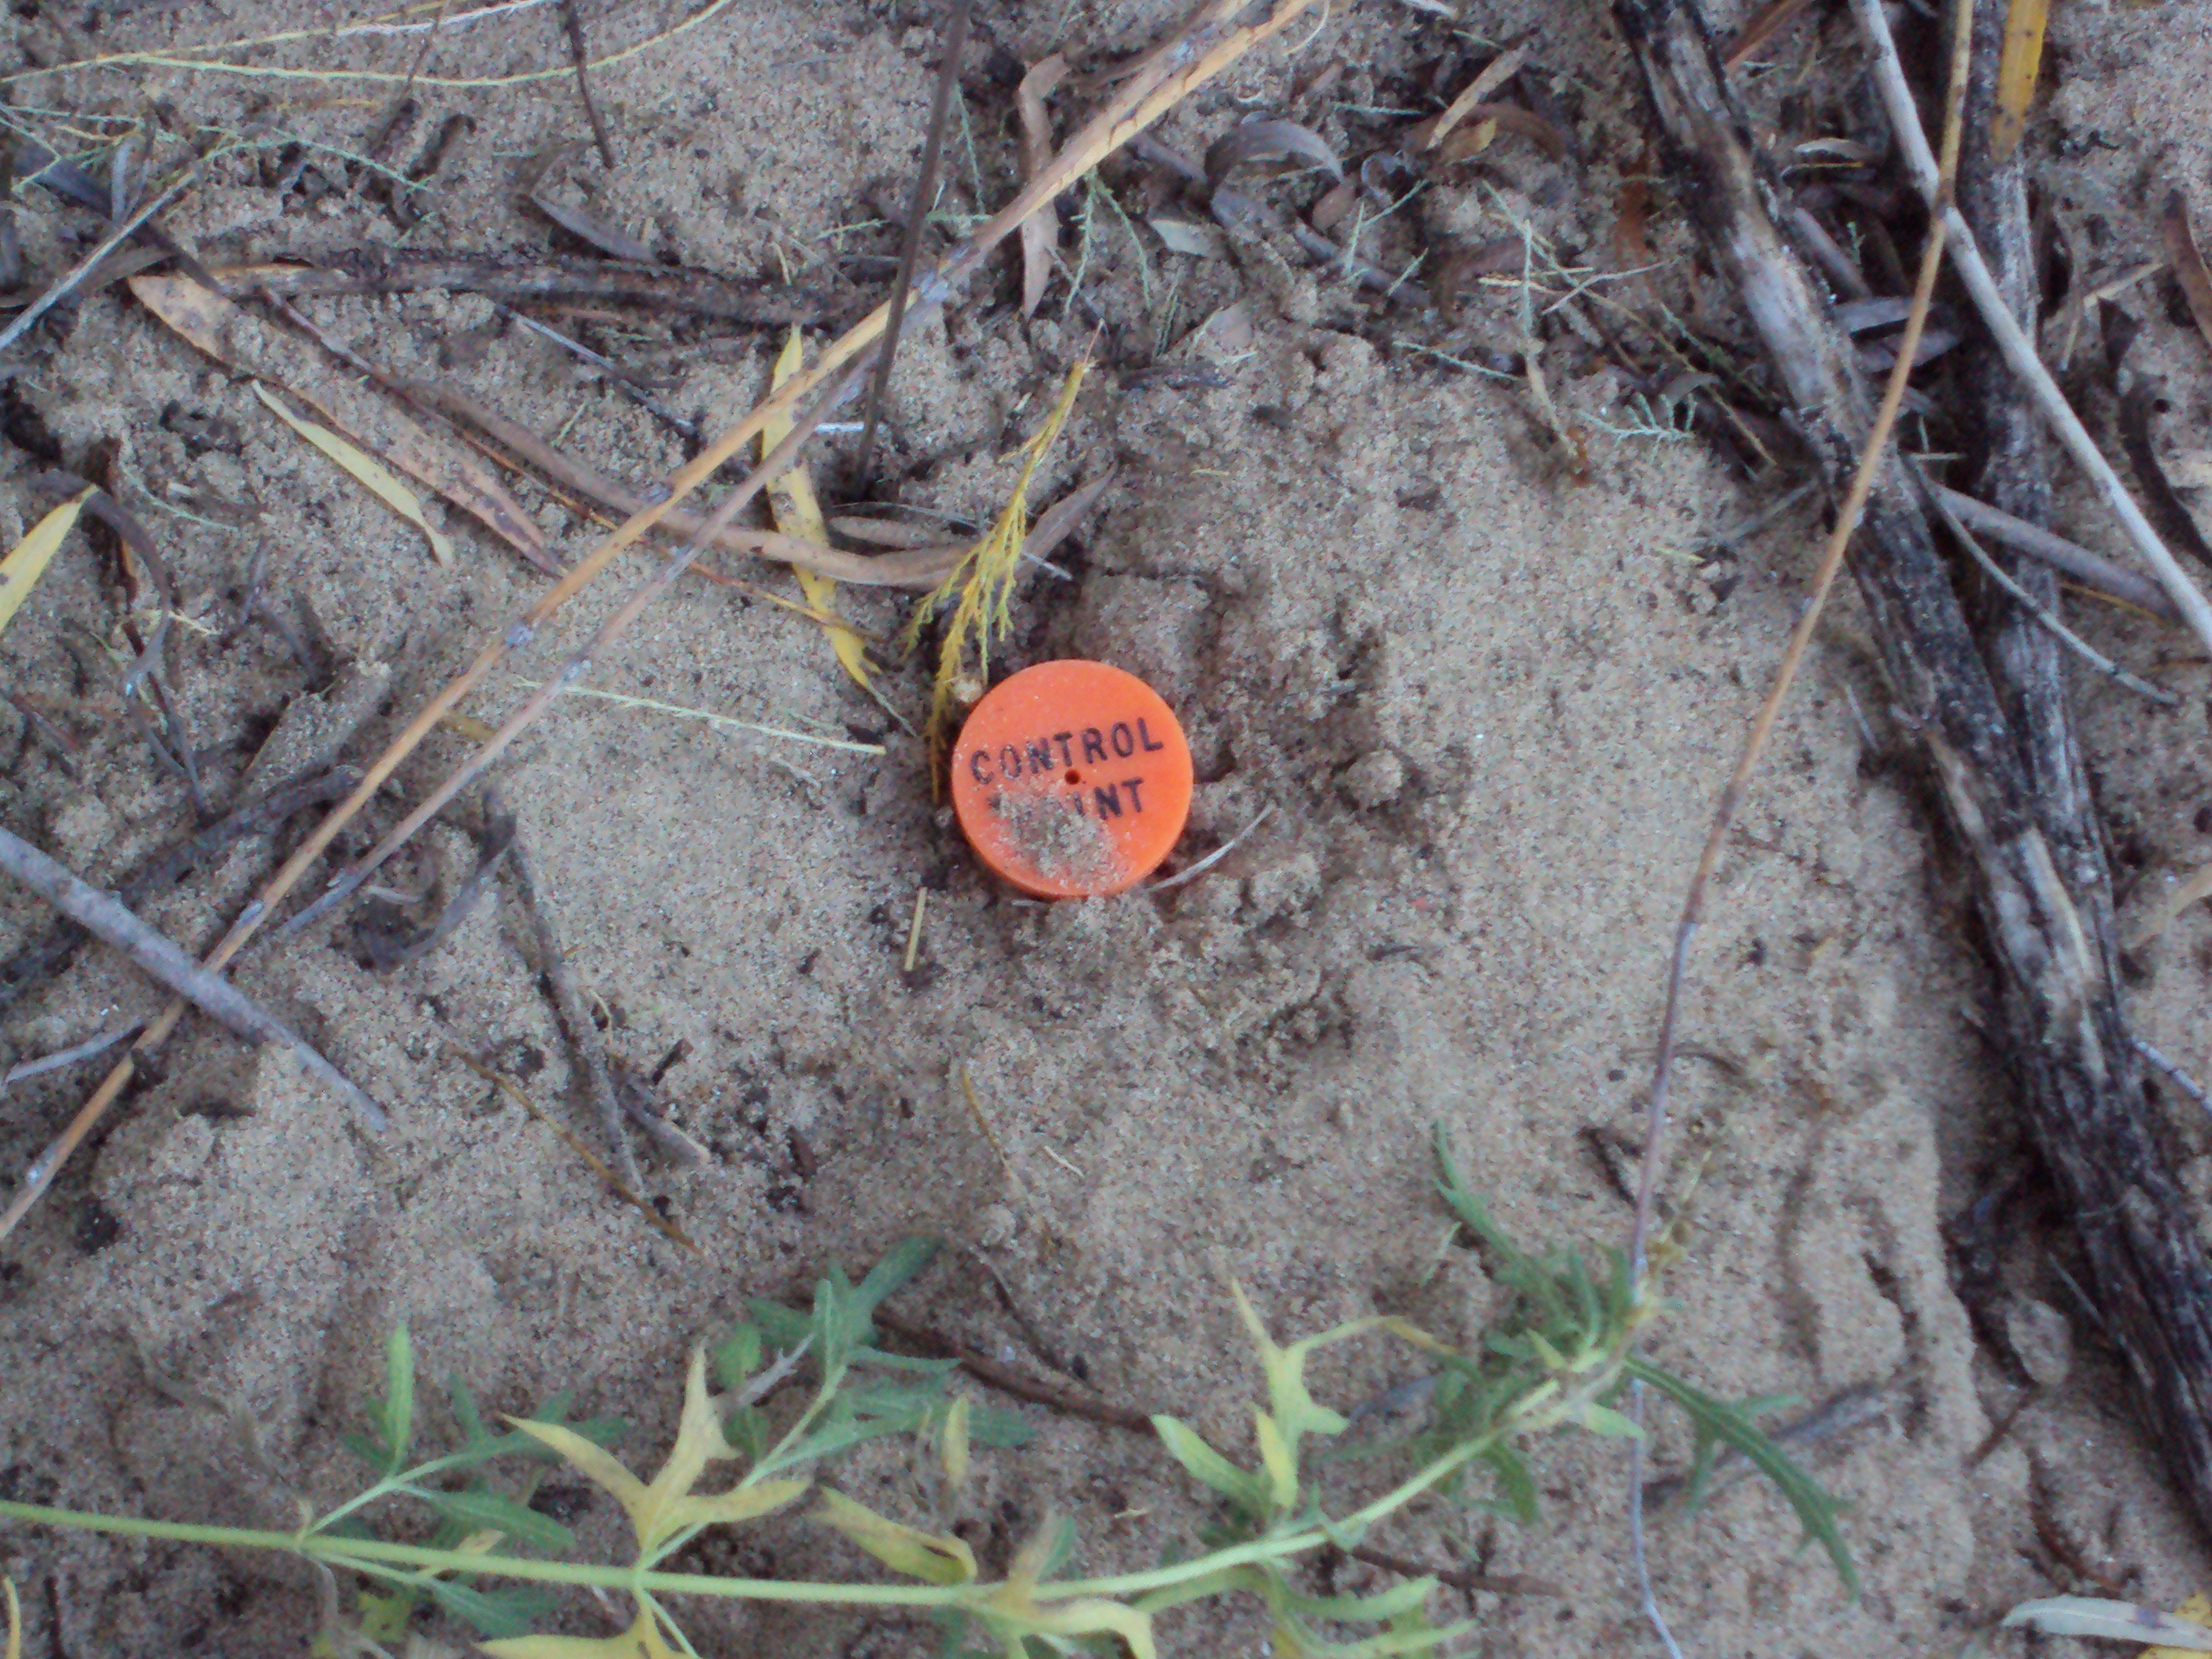
\includegraphics[width=3in]{Figures/Photo/ControlPoint}
	\caption[Typical plastic cap on rebar used to locate instrument location and back-sights.]{Typical plastic cap on rebar used to locate instrument location and back-sights.}
	\label{pic:plasticCap}
\end{figure}

A least squares fit linear regression equation was fit to the relative location of all points along the surveyed cross-section (Figure \ref{fig:SurveyPlanView}).  It was reasoned that a straight line through the data points would allow for a better approximation of the river's cross-section than connecting the points.  The straight line would represent a true cross-section, whereas connecting the points would exaggerate the distance across the cross-section.  The relative locations of the points as projected onto the best-fit line were entered into computer aided design and drafting (CADD) software (Figure \ref{fig:SurveySection}).  Horizontal lines, spaced 0.03 m (0.1 ft) apart from the bottom of the channel to 1.5 m (5 ft) from the bottom, were drawn from edge of bank to edge of bank.  The vertical location of these lines was taken as the flow depth and the length of the line was taken as the river top width.

% Figure - Translate survey points to horizontal best fit line.
\begin{figure}[htbp]
\centering
	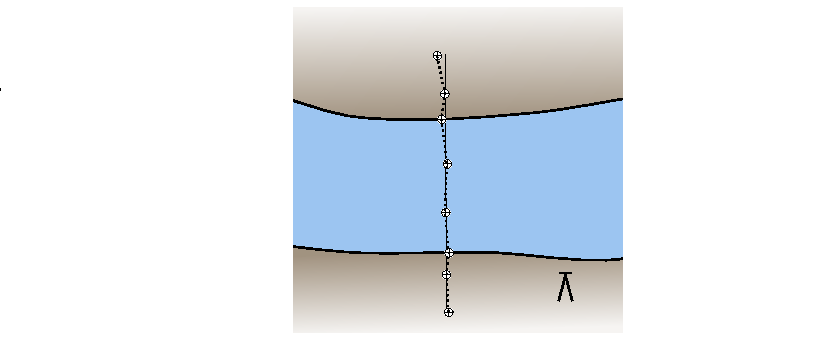
\includegraphics[width=6in]{Figures/LineDiagram/SurveyPlanView}
	\caption[Depiction of the conversion of River Survey Locations to Linear Cross-Section.]{Depiction of the conversion of River Survey Locations to Linear Cross-Section.  The crossed circles are the surveyed points.  The instrument (total station) is in the lower right-hand corner.  The dotted line depicts the cross section if no correction were made to linearize the survey cross section locations.  The solid line is the cross-section line created from the best-fit line through the surveyed points.  Surveyed points were translated perpendicular to the cross-section line to lie on the cross-section line across the river.}
	\label{fig:SurveyPlanView}
\end{figure}

% Figure - CADD drawing of cross section with no vertical exageration
\begin{figure}[htbp]
\centering
	\includegraphics[width=6in]{Figures/LineDiagram/USS1Trim}
	\caption[River Cross-Section as Draw in CADD Software.]{River Cross-Section as Draw in CADD Software.  The black line is the channel cross-section with the left side representing the north bank of the Arkansas River (water flow is into the page).  The blue horizontal line is the lowest point in the surveyed channel.  All elevations were shifted such that the bottom point had a stream depth of zero.  This particular cross section is at cross-section USS1.  The horizontal and vertical scales are identical.}
	\label{fig:SurveySection}
\end{figure}

%Each surveyed point had two location value sets.  The first set being relative to the instrument without location and orientation corrections.  The second set being relative to the State Plane with corrections for location, orientation, and elevation.  The two data sets shall be referred to as relative location and State Plane location, respectively.  The State Plane location for each point is directly derived from the relative location.  All survey error corrections were applied to the relative locations before converting the data to State Plane locations.
%
%Location errors due to GPS accuracy issues were corrected by comparing the State Plane location of the two back-sights to the GPS surveyed location at those sights.  The average difference in northing, easting, and elevation between the GPS back-sight coordinates and the instrument surveyed coordinates was used to shift the State Plane location of the instrument.  The State Plane location of all points was re-calculated after performing this correction.

\clearpage{}
\section{Data Compiled from Other Sources}
\label{sec:data collected by other sources}
The data collected in the field constituted a small portion of the total data required to perform water and mass balance calculations.  Additional data were obtained from three sources: the USGS, the CDWR, and the Colorado Climate Center (CCC).

The USGS operates and maintains the largest network of stream gauges in the United States.  USGS gauges in the LARV in Colorado are operated and maintained by the USGS Colorado Water Science Center.  Their main office is Lakewood, Colorado, with one of their satellite offices in Pueblo, Colorado.  Of the gauges listed in Tables \ref{tab:USRGauges} and \ref{tab:DSRGauges} and shown in Figures \ref{map:USRGaugeLocations} and \ref{map:DSRGaugeLocations}, five are operated by the USGS.  There is additional sensing equipment owned and maintained by the USGS at some stream gauges owned and operated by the CDWR.  Water temperature, air temperature, precipitation, and EC are the additional parameters typically measured and recorded by this equipment.  EC is reported as specific conductance standardized to \SI{25}{\degreeCelsius} and is the standard for EC used throughout this thesis.  EC values are reported in units of micro-siemens per centimeter (\si{\micro\siemens\per\centi\meter}) and are converted to units of deci-siemens per meter (\si{\deci\siemens\per\meter}).

% Map - USR stream gauge locations
\afterpage{%
	\clearpage%
	\begin{landscape}
		\begin{figure}[htbp]
			\centering
			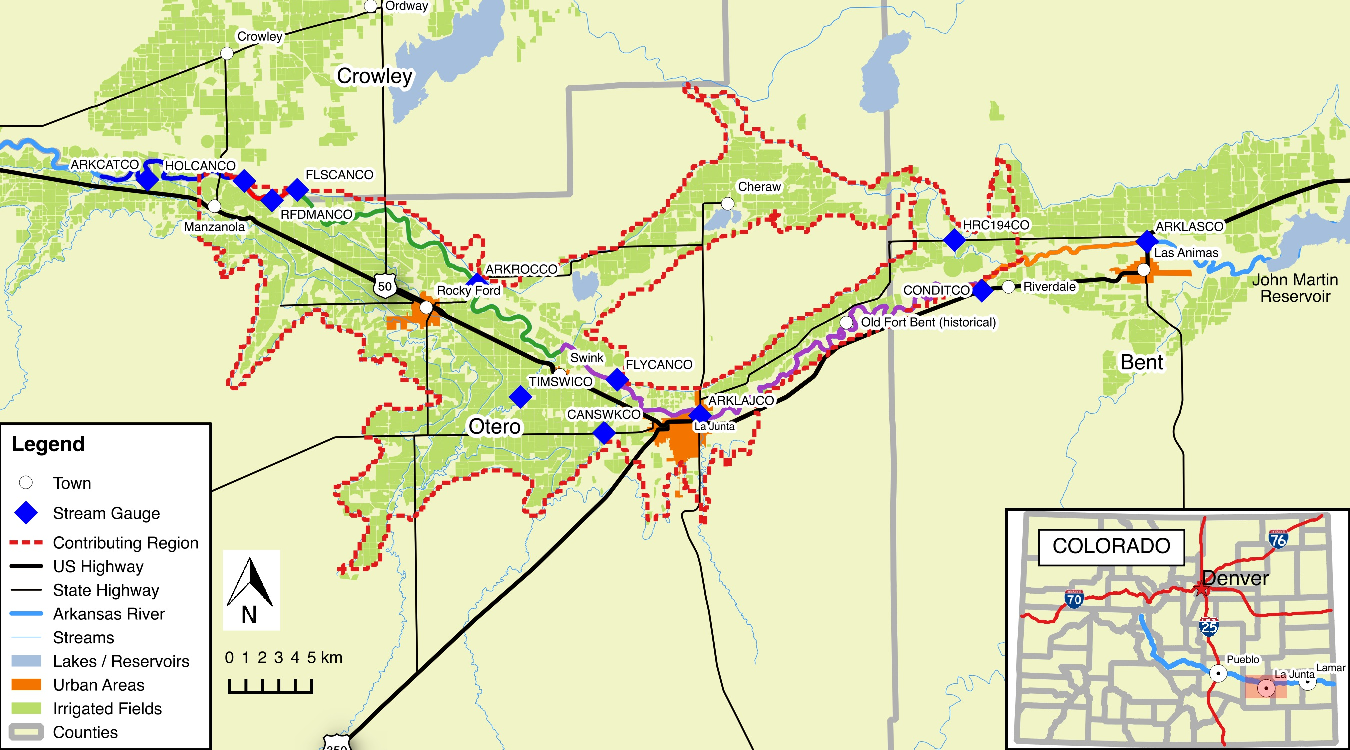
\includegraphics[scale=1]{Figures/Map/USRGauge}
			\caption[USR River and Tributary Stream Gauge Locations.]{USR River River and Tributary Stream Gauge Locations.}
			\label{map:USRGaugeLocations}
		\end{figure}
	\end{landscape}
}

% Map - DSR stream gauge locations
\afterpage{%
	\clearpage%
	\begin{landscape}
		\begin{figure}[htbp]
			\centering
			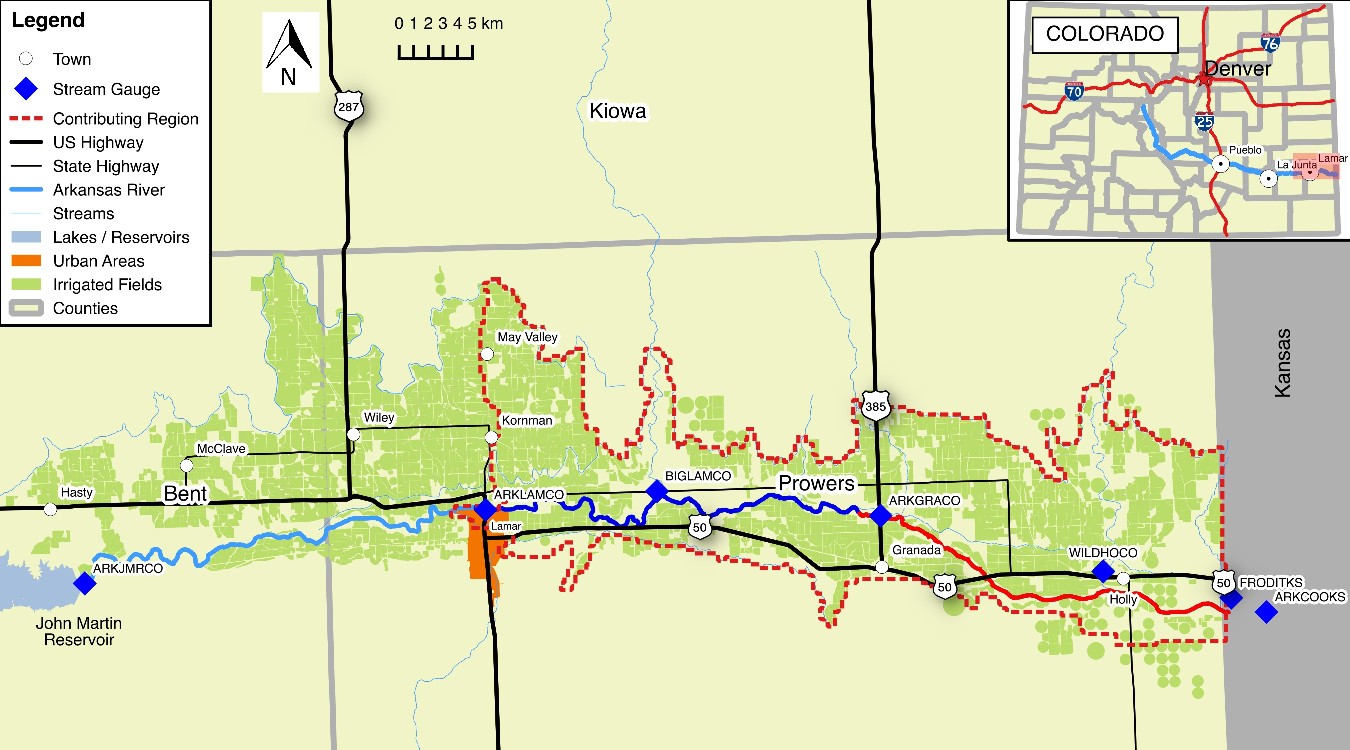
\includegraphics[scale=1]{Figures/Map/DSRGauge}
			\caption[DSR River and Tributary Stream Gauge Locations.]{DSR River River and Tributary Stream Gauge Locations.}
			\label{map:DSRGaugeLocations}
		\end{figure}
	\end{landscape}
}



% Table - USR stream gauge locations
\begin{table}[htbp]
\centering
  \caption[Upstream Study Region (USR) Stream Gauge Information.]{Upstream Study Region (USR) Stream Gauge Information.  Segment stream gauges record flow depth for surface area and river volume change calculations.  A value of zero (0) indicates the location of the segment stream gauge.  Negative distances indicate the point is upstream of the reference stream gauge location. Segment B does not contain a stream gauge on the river main stem.}
    \label{tab:USRGauges}
\begin{tabular}{ccccccc}
	\toprule
	                      River                       &     CDWR     &     USGS     &  \multicolumn{2}{c}{Dist. from}  &  \multicolumn{2}{c}{Dist. from}   \\
	                     Segment                      & Stream Gauge & Stream Gauge & \multicolumn{2}{c}{USR Upstream} & \multicolumn{2}{c}{River Segment} \\
	                      Name                        &     Name     &     Name     &   \multicolumn{2}{c}{Boundary}   & \multicolumn{2}{c}{Stream Gauge}  \\
	\cmidrule(r{.5em}l){4-5} \cmidrule(r{.5em}l){6-7} &              &              &  mi  &            km             &  mi  &             km             \\ \toprule
	               \multirow{2}{*}{A}                 &   ARKCATCO   &              & 2.7  &            4.3            &  0   &             0              \\
	                                                  &   HOLCANCO   &              & 7.8  &           12.6            & 5.1  &            8.2             \\ \midrule
	               \multirow{2}{*}{B}                 &   RFDMANCO   &              & 9.2  &           14.8            &      &  \\
	                                                  &   FLSCANCO   &              & 10.2 &           16.4            &      &  \\ \midrule
	               \multirow{4}{*}{C}                 &   RFDRETCO   &              & 11.7 &           18.8            & -8.5 &           -13.7            \\
	                                                  &   ARKROCCO   &              & 20.2 &           32.5            &  0   &             0              \\
	                                                  &   TIMSWICO   &   7121500    & 26.1 &            42             & 5.9  &            9.5             \\
	                                                  &   FLYCANCO   &              & 29.3 &           47.2            & 9.1  &            14.6            \\ \midrule
	               \multirow{3}{*}{D}                 &   CANSWKCO   &              & 30.3 &           18.8            & -3.5 &            -5.6            \\
	                                                  &   ARKLAJCO   &              & 33.8 &           54.4            &  0   &             0              \\
	                                                  &   CONDITCO   &              & 52.8 &            85             &  19  &            30.6            \\ \midrule
	               \multirow{2}{*}{E}                 &   HRC194CO   &              & 55.1 &           88.7            & -6.6 &           -10.6            \\
	                                                  &   ARKLASCO   &   7124000    & 61.7 &           99.3            &  0   &             0              \\ \bottomrule
\end{tabular}
\end{table}

% Table - DSR stream gauge locations
\begin{table}[htbp]
  \centering
  \caption[Downstream Study Region (DSR) Stream Gauge Information.]{Downstream Study Region (DSR) Stream Gauge Information.  River segment stream gauges record flow depth for surface area and river volume change calculations.  A value of zero (0) indicates the location of the segment stream gauge.  Negative distances indicate the point is upstream of the reference stream gauge location. Stream gauges ARKJMRCO, FRODITKS and ARKCOOKS although required for analysis, are not within the DSR.}
\label{tab:DSRGauge}
\begin{tabular}{ccccccc}
	\toprule
	                       River                        &     CDWR     &     USGS     &  \multicolumn{2}{c}{Dist. from}  &  \multicolumn{2}{c}{Dist. from}   \\
	                      Segment                       & Stream Gauge & Stream Gauge & \multicolumn{2}{c}{DSR Upstream} & \multicolumn{2}{c}{River Segment} \\
	                       Name                         &     Name     &     Name     &   \multicolumn{2}{c}{Boundary}   & \multicolumn{2}{c}{Stream Gauge}  \\
	\cmidrule(r{0.5em}l){4-5} \cmidrule(r{0.5em}l){6-7} &              &              &  mi  &            km             &  mi  &             km             \\ \toprule
	                                                    &   ARKJMRCO   &   07130500   & -22  &           -35.4           &      &  \\ \midrule
	                \multirow{3}{*}{F}                  &   ARKLAMCO   &   07133000   &  0   &             0             &  0   &             0              \\
	                                                    &   BIGLAMCO   &   07134100   & 11.6 &           18.7            & 11.6 &            18.7            \\
	                                                    &   BUFDITCO   &              & 23.4 &           37.7            & 23.4 &            37.7            \\ \midrule
	                \multirow{2}{*}{G}                  &   ARKGRACO   &   07134180   & 24.9 &           40.1            &  0   &             0              \\
	                                                    &   WILDHOCO   &   07134990   & 38.1 &           61.3            & 13.2 &            21.2            \\ \midrule
	                                                    &   FRODITKS   &   07137000   & 43.5 &            70             &      &  \\
	                                                    &   ARKCOOKS   &   07137500   & 43.2 &           74.4            &      &  \\ \bottomrule
\end{tabular}
\end{table}

The USGS and CDWR do not have typical gauge sites in the LARV.  Gauge housing and locations vary as show in Figure \ref{pic:Housings}.  These figures are not all inclusive and other variations occur in the LARV.  Both agencies were consistent in the flow measuring equipment deployed to the gauge sites.  During the Se sampling time frame, all stream gauges were constant flow bubblers as described in the USGS Techniques of Water Resources Investigations (TWRI) Report, Book 3, Section A, Chapter 7 \parencite{USGS2010TWRI}.  After all Se sampling was completed, the USGS and CDWR began upgrading some of the gauge sites with radar non-contact water level sensors.  It is unknown how this will affect the comparison of the results of this thesis with any future work.

% Picture - gauge houseings in LARV
\begin{figure}[htbp]
\centering
	\begin{subfigure}[t]{0.5\textwidth}
		\centering
		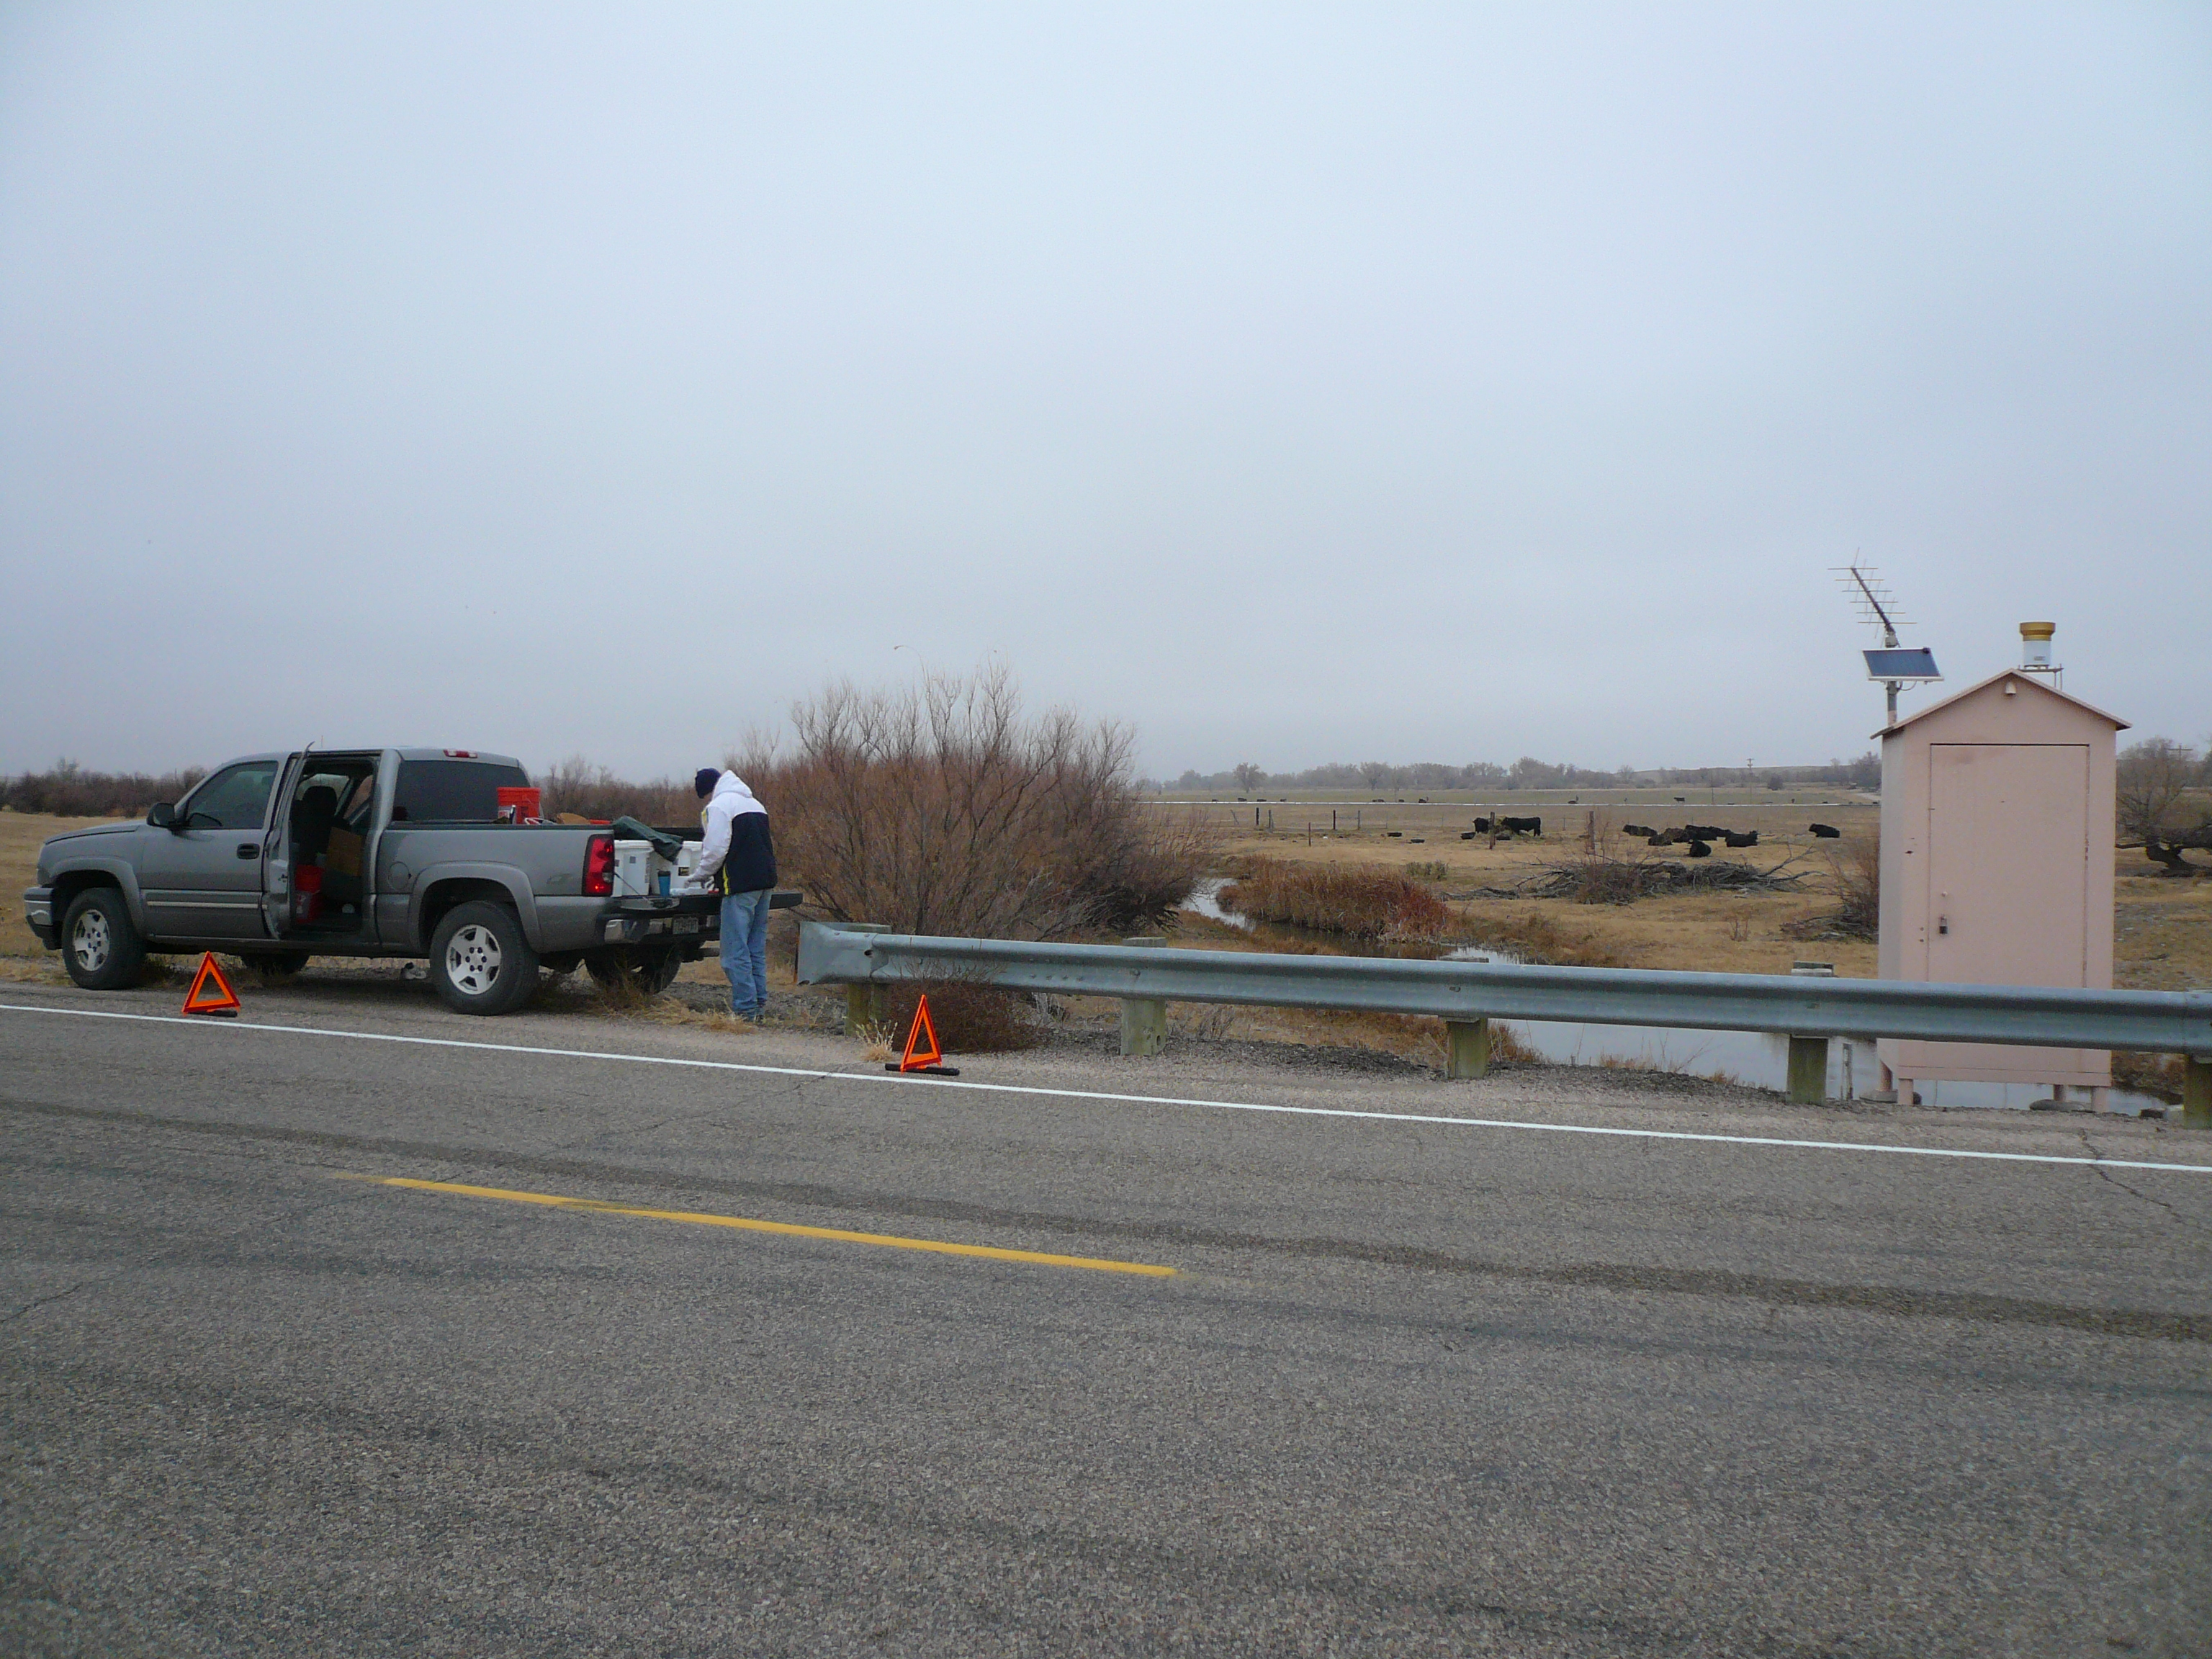
\includegraphics[width=2.9in]{Figures/Photo/GaugeSite1}
		\caption{HRC194CO.}
	\end{subfigure}%
	~
	\begin{subfigure}[t]{0.5\textwidth}
		\centering
		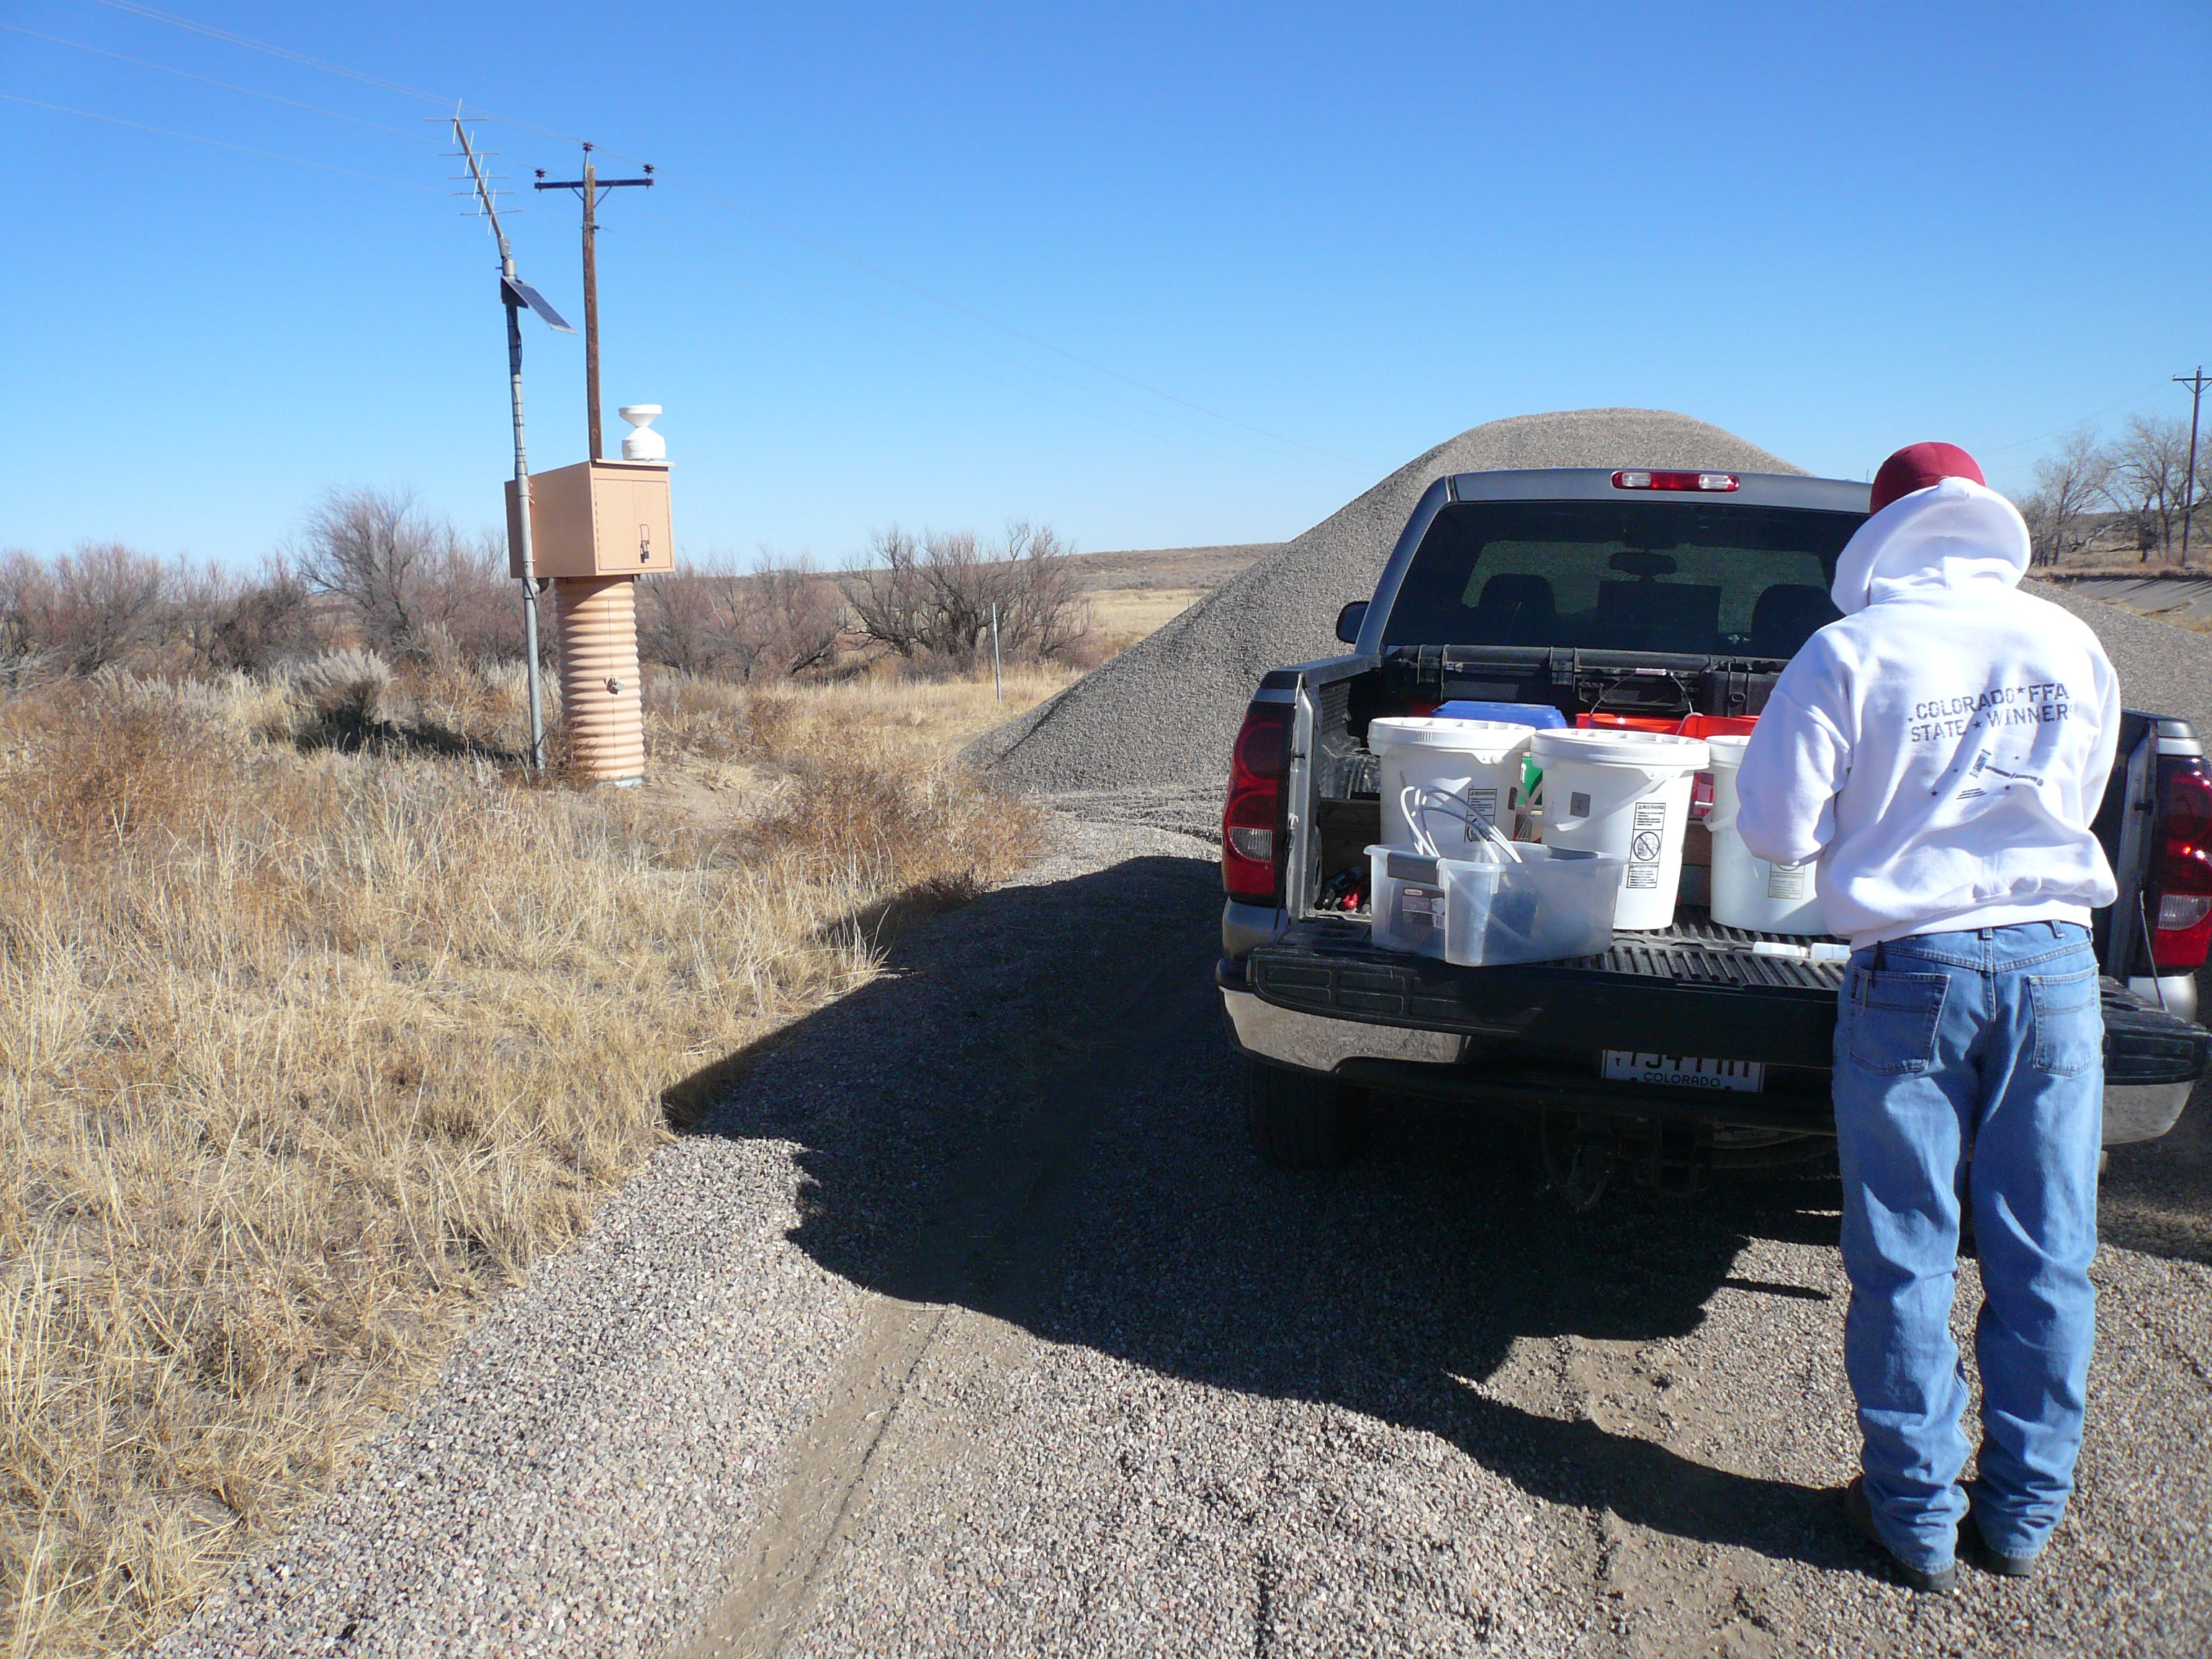
\includegraphics[width=2.9in]{Figures/Photo/GaugeSite2}
		\caption{BIGLAMCO.}
	\end{subfigure}

	\begin{subfigure}[t]{0.5\textwidth}
		\centering
		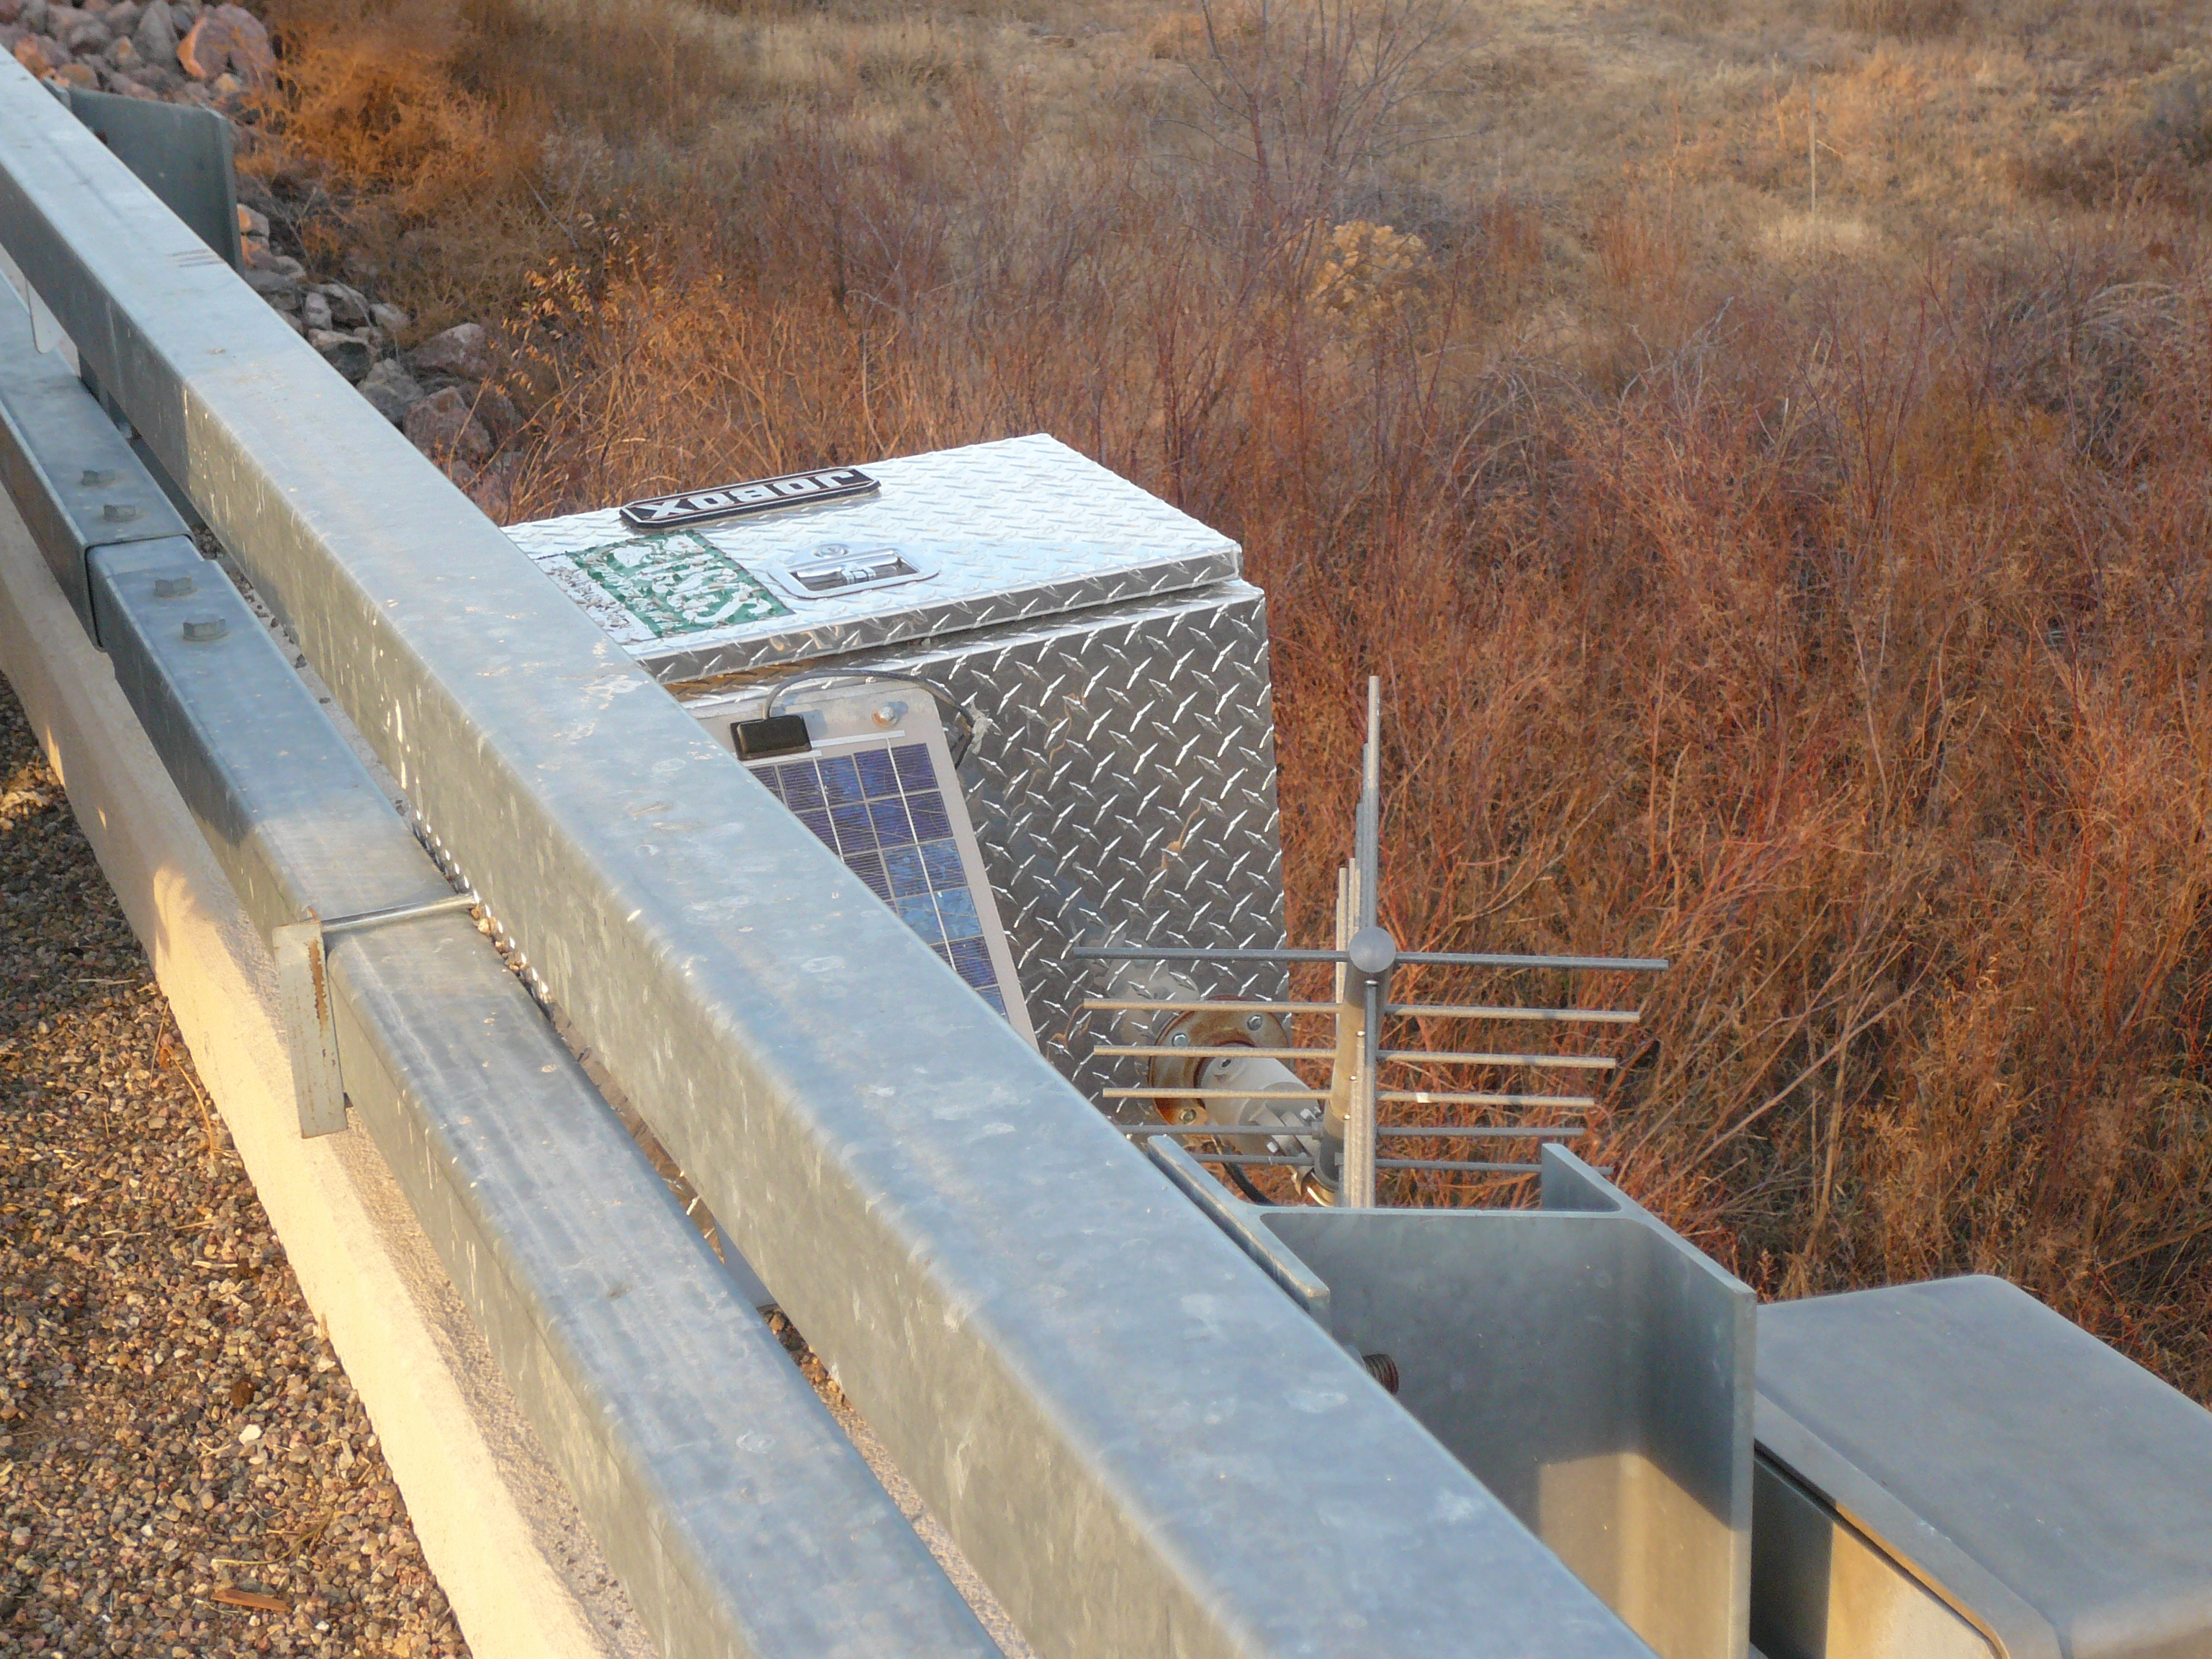
\includegraphics[width=2.9in]{Figures/Photo/GaugeSite3}
		\caption{TIMSWICO}
	\end{subfigure}%
	~
	\begin{subfigure}[t]{0.5\textwidth}
		\centering
		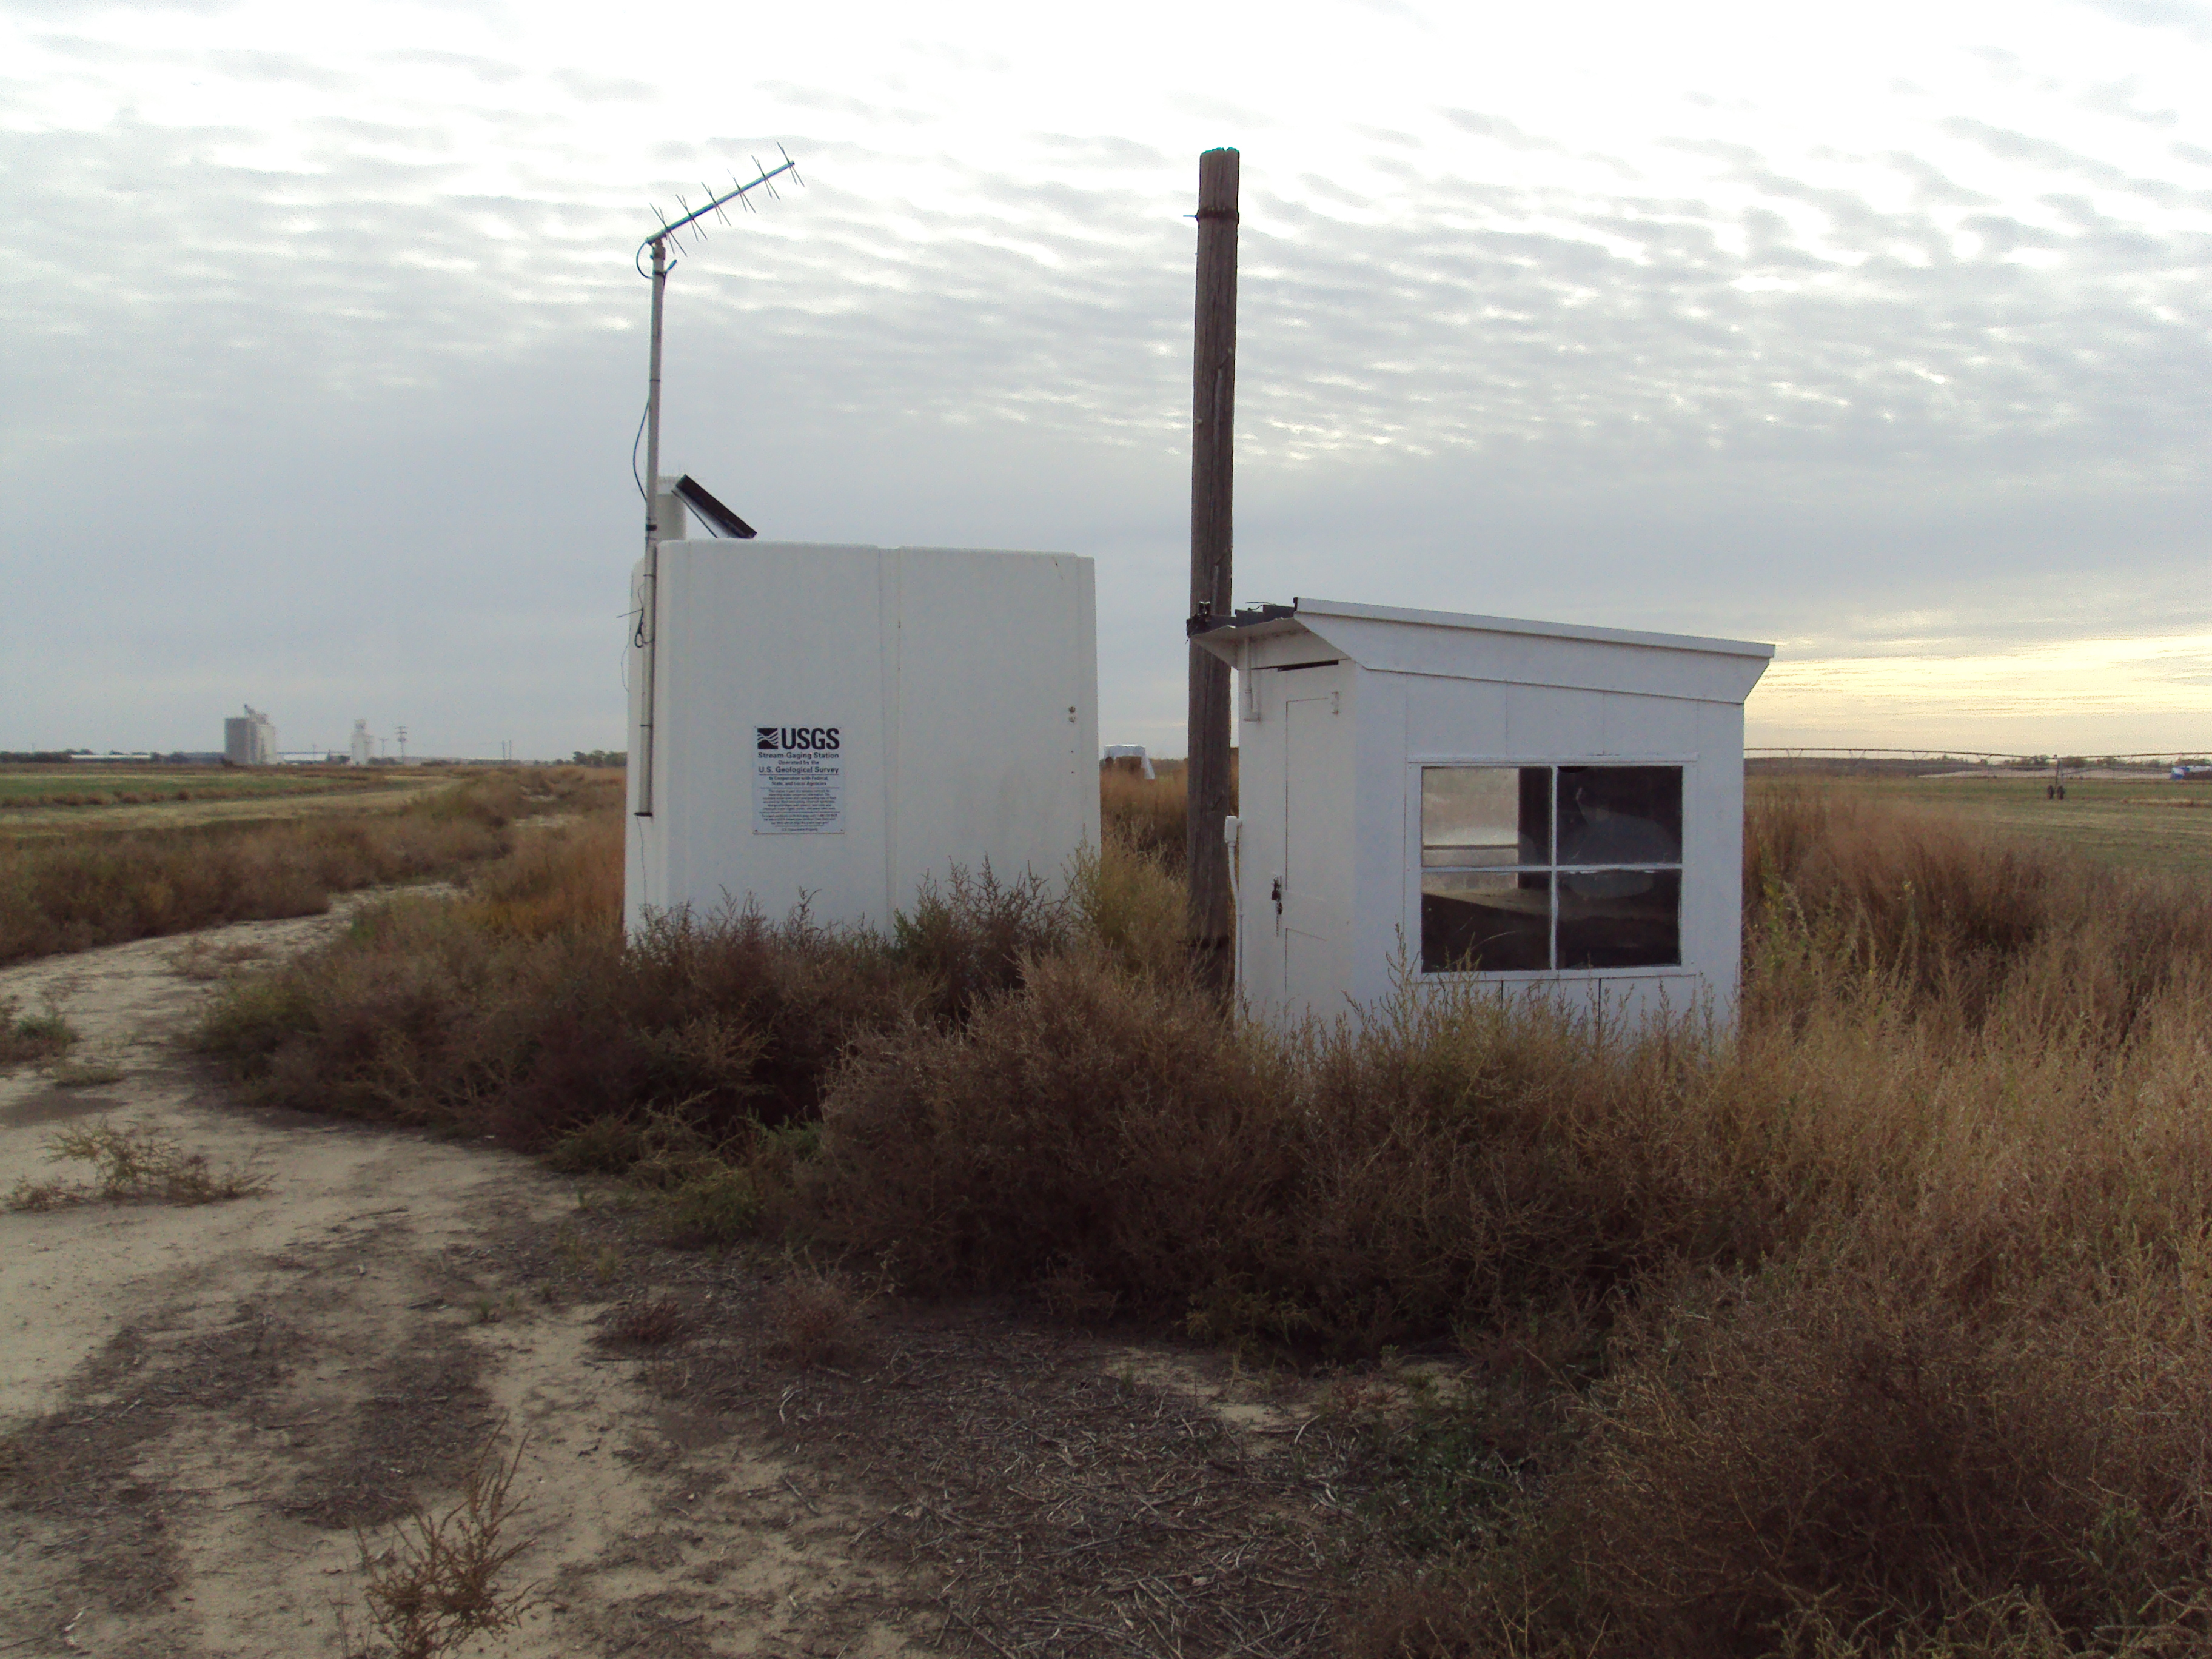
\includegraphics[width=2.9in]{Figures/Photo/GaugeSite4}
		\caption{FRODITKS}
	\end{subfigure}
	
	\begin{subfigure}[t]{0.5\textwidth}
		\centering
		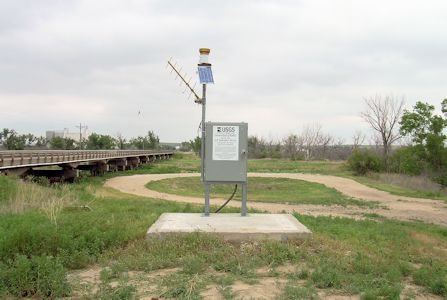
\includegraphics[width=2.9in]{Figures/Photo/GaugeSite6}
		\caption{ARKCOOKS}
	\end{subfigure}%
	\caption[Range of Stream Gauge Equipment Housings in the LARV.]{Range of Stream Gauge Equipment Housings in the LARV.}
	\label{pic:Housings}
\end{figure}

Data from the CDWR and USGS stream gauges are reported on web sites operated by the two agencies.  Table \ref{tab:gauge other data} lists the gauge sites used in this study and notes the additional data besides streamflow collected at each gauge.  Additional data are reported by the agency that owns and operates the gauge site.  USGS instruments at a CDWR gauge site are recorded and reported on the CDWR web site.  Note that the CDWR gauge site ARKLAMCO, which is owned by the USGS, does not have any additional data collection instruments.

% Table - USR stream gauge data
\begin{table}[htbp]
  \centering
  \caption[Summary of Stream Gauges with Notation of Additional Data Collected.]{Summary of Stream Gauges with Notation of Additional Data Collected.}
  \label{tab:gauge other data}
  \begin{tabular}{cccccc}
  	\toprule
  	        Study         & \multicolumn{2}{c}{Stream Gauge ID} & \multicolumn{3}{c}{Parameter} \\
  	        Reach         &   CDWR    &          USGS           & Air Temp. & Water Temp. & EC  \\ \toprule
  	\multirow{12}{*}{USR} & ARKCATCO  &                         &           &      X      &  X  \\
  	                      & HOLCANCO  &                         &           &             &  \\
  	                      & RFDMANCO  &                         &           &             &  \\
  	                      & FLSCANCO  &                         &           &             &  \\
  	                      & RFDRETCO  &                         &           &             &  \\
  	          %           & ARKROCCO  &                         &           &      X      &  X  \\
  	                      & TIMSWICO  &                         &           &             &  \\
  	                      & FLYCANCO  &                         &           &             &  \\
  	                      & CANSWKCO  &                         &           &             &  \\
  	                      & ARKLAJCO  &                         &     X     &             &  \\
  	                      & CONDITCO  &                         &           &             &  \\
  	                      & HRC194CO  &                         &           &             &  \\
  	                      & ARKLASCO  &        07124000         &           &      X      &  X  \\ \midrule
  	\multirow{7}{*}{DSR}  & ARKJMRCO  &        07130500         &           &      X      &  X  \\
  	                      & ARKLAMCO  &        07124000         &           &             &  \\
  	                      & BIGLAMCO  &                         &           &             &  \\
  	                      & BUFDITCO  &                         &           &             &  \\
  	          %           & ARKGRACO  &        07134180         &           &             &  \\
  	                      & WILDHOCO  &                         &           &             &  \\
  	                      & FRODITCKS &                         &           &             &  \\
  	                      & ARKCOOKS  &        07137500         &           &      X      &  X  \\ \bottomrule
  \end{tabular}
\end{table}

Stream flow data were obtained as average daily flow for each stream gauge. Some average daily flow records were reported as being estimated or provisional.  These data points were removed from the analysis.  Average daily flow data were quality checked for unacceptable values.  For each gauge, acceptable values were defined as those above zero and below the 99th percentile of all flows recorded at that gauge.  Unacceptable values were removed from the data set.

All stream gauges report gauge height which is the vertical distance from the gauge site datum to the water surface (Figure \ref{fig:VariableChannel}).  Gauge site datum is arbitrarily set, but is tied to a local survey benchmark.  Flow depth is the depth from the bottom of the channel to the water's surface.  While both gauge height and flow depth measure the distance to the water's surface, their datums can, and frequently do vary.  The Arkansas River is a shifting bed channel and as such, the channel bottom elevation varies with time at a gauge site.  The rating table, which is used to convert flow depth to flow rate, is configured such that flow depths below the channel bottom have a flow rate of zero.  The table is frequently updated with data obtained from routine re-calibration of the stream gauge.

% Figure - river cross section w/ variable channel bottom
\begin{figure}[htbp]
\centering
	\includegraphics[width=6in]{Figures/LineDiagram/XSectionSimple}
	\caption[Depiction of Variable Channel Bottom and Fixed Gauge Datum.]{Depiction of Variable Channel Bottom and Fixed Gauge Datum.  $ d_1 $ and $ d_2 $ are flow depths at different times.  $ h_i $ is the stream gauge height measurement at any time.}
	\label{fig:VariableChannel}
\end{figure}

Gauge height data is the directly measured value that is used to calculate flow rate.  Flow rates are calculated from gauge height using a gauge site specific rating table produced in accordance with USGS standards and procedures \parencite{USGS1982a, USGS1982b}.  Gauge heights for the USGS and CDWR gauges were obtained from the respective regional offices.  Historical recorded gauge heights are not reported on web sites as these data are considered to be precursors for stream flow rate calculations.  Stream gauge data were provided as both average daily gauge height and as recorded gauge height.  Recorded gauge height is the gauge height recorded in 15-minute increments during a calendar day.  Average daily gauge height is the mean of the recorded gauge heights over a calendar day.  All gauge heights were provided in units of feet above the gauge datum.  Gauge height units were converted to SI units of meters for this study to simplify calculations and discussion.  Gauge height data were checked for accuracy by the source agency before being released to CSU staff.

Water temperature data were obtained as average daily temperature or as minimum and maximum daily temperatures, depending on the gauge site.  Average daily temperature is calculated as the mean of the minimum and maximum daily temperature.  Water temperature data were provided in units of \si{\degreeCelsius}.  Since frozen or partially-frozen river channels do not have the same gauge height to flow rate relationship as free running river channels, data corresponding to water temperatures below zero were removed from the data set.

EC data obtained from USGS and CDWR stream gauge sites were provided as average daily values for each recording gauge station.  EC values recorded at the stations were compared to available EC values measured by CSU to cross-validate both data sets.  Gauge station recorded EC values were quality controlled by removing the bottom and top 1\% of EC values for each gauge.  Changes in average daily EC between consecutive days were checked for validity.  Changes greater than 33\% were analyzed to determine if the EC change was valid.  The average daily flow rate and time of year were taken into consideration when determining if the questionable EC values were valid.  EC values that exceeded the 33\% change but were accompanied by large changes in EC or during peak irrigation seasons were considered valid EC values.  Values considered to be invalid were removed from the data set.  EC values were provided in units of \si{\micro\siemens\per\centi\meter}.

Atmospheric data was required to determine the volume of water evaporated from the river's surface.  The Colorado Agricultural Meteorological Network (CoAgMet) was chosen as the source for atmospheric data.  The National Weather Service station sites in the study regions are located in populated areas or at airports and is only suitable for weather analysis.  CoAgMet station sites are more numerous, are located in agricultural areas, and are suitably equipped for evaporation and transpiration ($ET$) analysis.  An example of one of the weather stations is shown in Figure \ref{pic:CoAgMetStation}.  The CoAgMet network is operated by the Colorado Climate Center at CSU and consists of 86 weather stations throughout the state.  Some stations are only seasonally operational \parencite{Andales2009, Csu2012}.  Of the full-time sites, three are located in the USR and three are located in the DSR as shown in Figures \ref{map:USRCoAgMetLocations} and \ref{map:DSRCoAgMetLocations}, respectively. The CoAgMet weather stations in the USR are located such that they represent the upper, middle, and lower segments of the USR.  The CoAgMet stations in the DSR are more tightly grouped toward the upstream end of the reach, but still are considered representative of the study reach. The weather stations are primarily located in agricultural areas to provide agricultural researchers with data used for many different research applications.  The data also are available to the public through a web site.  This has aided farmers in determining irrigation timing and quantity \parencite{Andales2009}.  Table \ref{tab:CoAgMetInstruments} is a list of the parameters measured at the CoAgMet stations and the typical instruments used.  Not all stations are identical.  Instruments were replaced or upgraded by CCC staff when required with instruments that were available and equal to or better in quality than the instrument being replaced.

% Picture - CoAgMet weather station
\begin{figure}[htbp]
\centering
	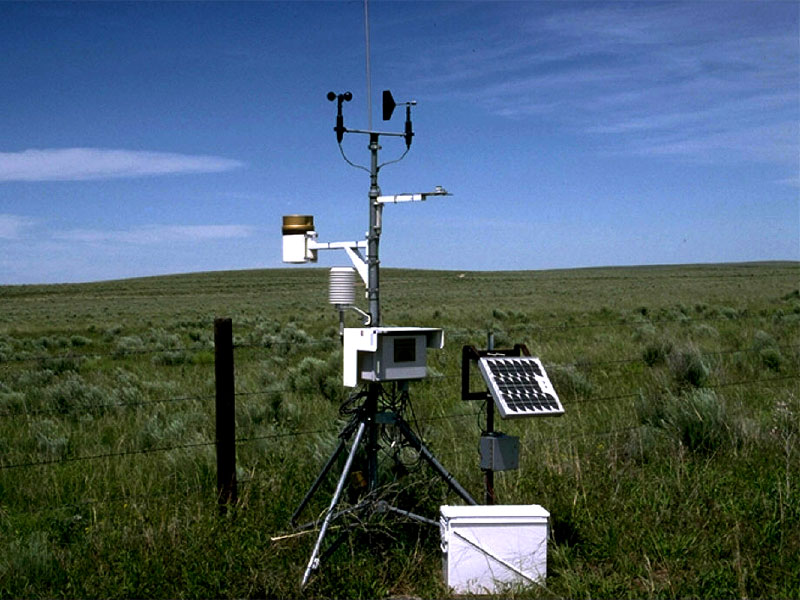
\includegraphics[width=4in]{Figures/Photo/CoagmetStation}
	\caption[Typical CoAgMet Weather Station.]{Typical CoAgMet Weather Station.}
	\label{pic:CoAgMetStation}
\end{figure}


% Map - USR CoAgMet weather station locations
	\begin{landscape}
	\begin{figure}[htbp]
		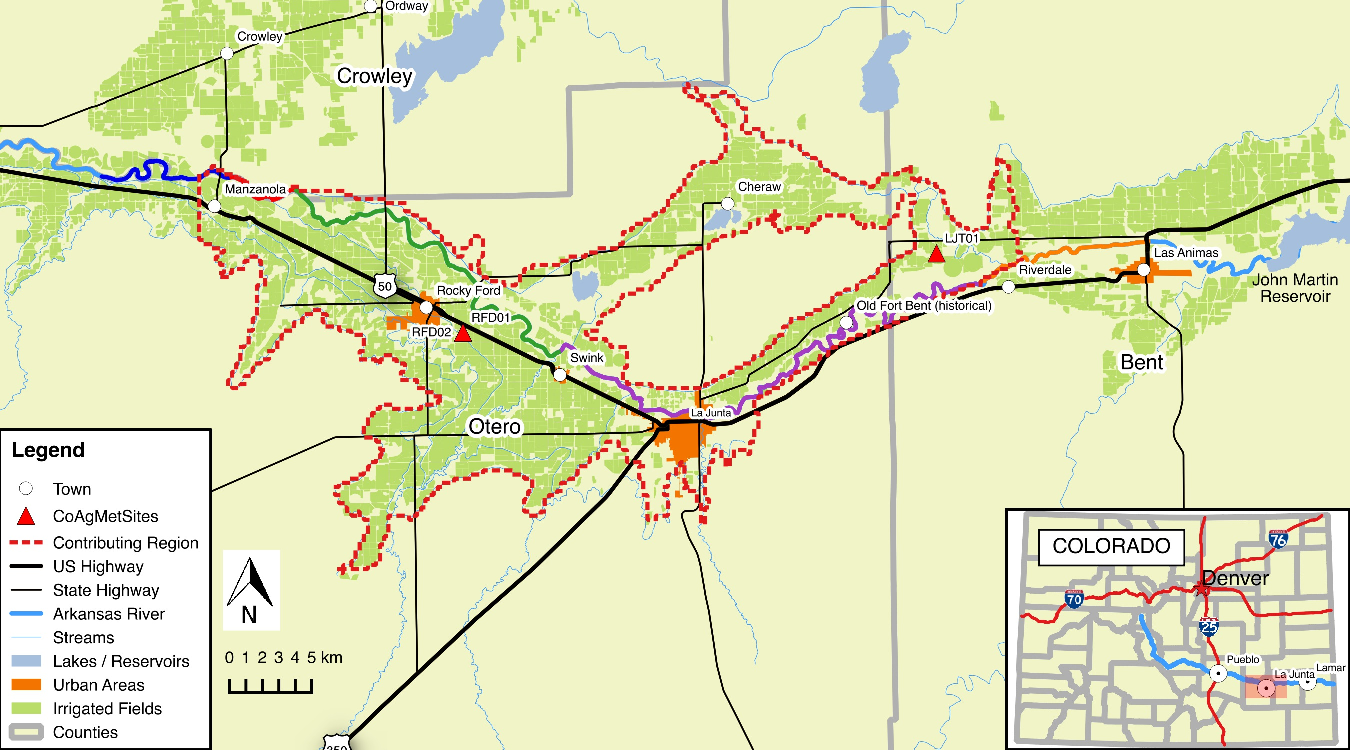
\includegraphics[scale=1]{Figures/Map/USRCoAgMet}
		\caption[USR CoAgMet Weather Station Locations.]{USR CoAgMet Weather Station Locations.}
		\label{map:USRCoAgMetLocations}	
	\end{figure}
	\end{landscape}

% Map - DSR CoAgMet weather station locations
	\begin{landscape}
	\begin{figure}[htbp]
		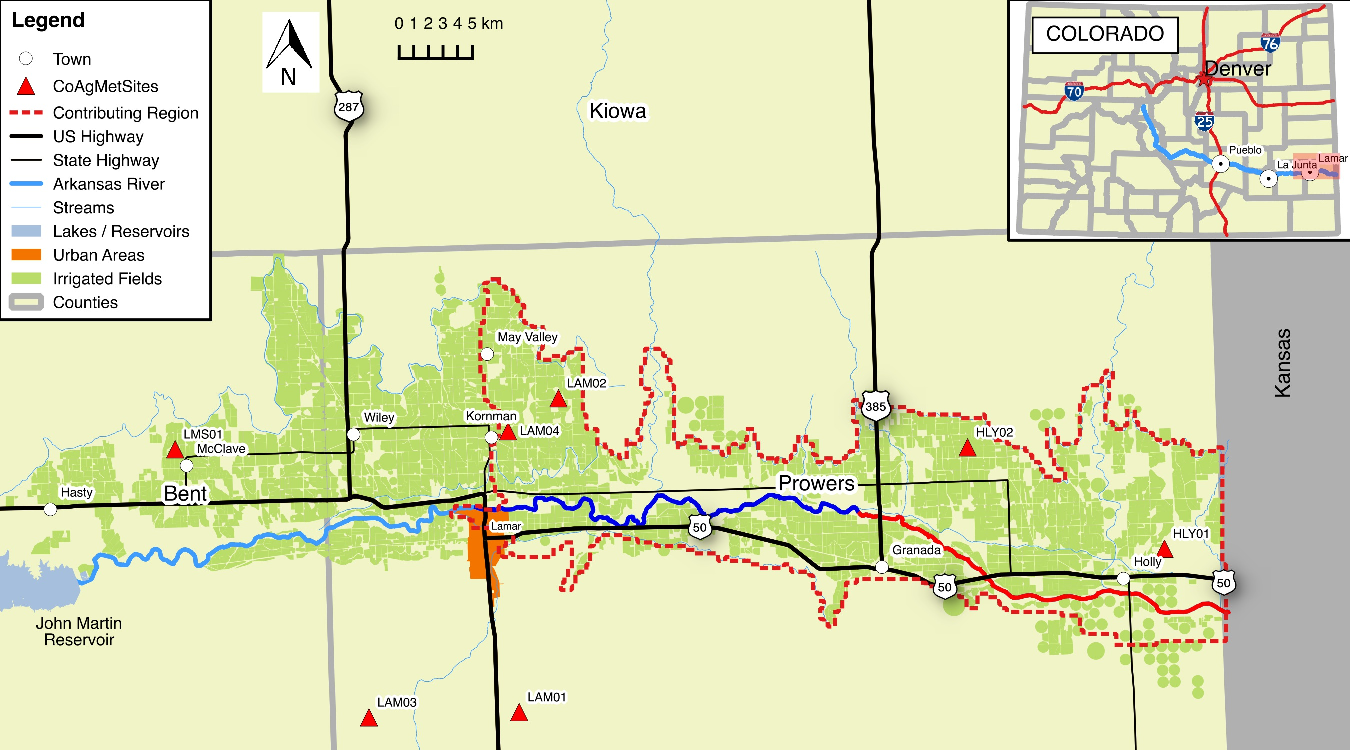
\includegraphics[scale=1]{Figures/Map/DSRCoAgMet}
		\caption[DSR CoAgMet Weather Station Locations.]{DSR CoAgMet Weather Station Locations.}
		\label{map:DSRCoAgMetLocations}	
	\end{figure}
	\end{landscape}
 
% Table - Typical instruments at CoAgMet station
\begin{table}[htbp]
\centering
\caption[Typical Instrumentation at CoAgMet Weather Stations.]{Typical Instrumentation at CoAgMet Weather Stations.}
\label{tab:CoAgMetInstruments}
\begin{tabular}{c c}
	\toprule
	       Measured Parameter        & Typical Instrument                          \\ \toprule
	Temperature \& Relative Humidity & Vaisala HMP45C Probe                        \\
	              Wind               & R.M. Young Wind Sentry                      \\
	        Solar Radiation          & Licor LI-200X Pyranometer                   \\
	         Precipitation           & TE525 tipping bucket raingauge              \\
	        Soil Temperature         & CSI Model 107 Soil Temp Probe (thermistor)  \\
	          Data Loggers           & Campbell Scientific CR10, CR10X, and CR1000 \\ \bottomrule
\end{tabular}
\end{table}

Table \ref{tab:CoAgMet} lists the weather stations in the LARV that were used in this study.  This table lists the station name and location, the state of irrigation of the land surrounding the site, the date of first record, and a comparative estimate of the site estimated $ET_{ref}$ to the actual $ET_{ref}$.  The irrigation state of the land surrounding the site is used to determine the comparative estimate of the site estimated $ET_{ref}$ to the actual  $ET_{ref}$.  If the monitoring station is on irrigated land then the $ET_{ref}$ values calculated based on site data are expected to be at or near the actual value of $ET_{ref}$ for the site.  If the station is on dry, or non-irrigated land, then calculated $ET_{ref}$ values tend to over estimate the actual $ET_{ref}$.

% Table - CoAgMet stations used in analysis
\begin{table}[htb]
  \centering
  \caption[CoAgMet Weather Stations used for analysis in the LARV.]{CoAgMet Weather Stations used for analysis in the LARV.}
  \label{tab:CoAgMet}
    \begin{tabular}{ccccccc}
    	\toprule
    	                         &                           &                                &                &                             &                                 &        Comparative        \\
    	         Study           &                        \multicolumn{3}{c}{Station }                         & \multirow{2}{*}{Irrigation} &             Date of             &          Est. of          \\
    	\cmidrule{2-4}
    Reach &            ID             &              Name              &    Location    &                             &          First Record           &          Site ET          \\ \toprule
    	\multirow{7}[0]{*}{USR}  & \multirow{2}[0]{*}{FWL01} &   \multirow{2}[0]{*}{Fowler}   &  Fowler Golf   &  \multirow{2}[0]{*}{Full}   & \multirow{2}[0]{*}{17 Mar 2005} &  \multirow{2}[0]{*}{--}   \\
    	                         &                           &                                &     Course     &                             &                                 &  \\
    	     \cmidrule{2-7}      & \multirow{2}[0]{*}{LJT01} &  \multirow{2}[0]{*}{LaJunta}   &    11 mi NE    &  \multirow{2}[0]{*}{Full}   & \multirow{2}[0]{*}{17 Mar 2005} & \multirow{2}[0]{*}{Under} \\
    	                         &                           &                                &   of LaJunta   &                             &                                 &  \\
    	     \cmidrule{2-7}      & \multirow{3}[0]{*}{RFD01} & \multirow{3}[0]{*}{RockyFord}  & CSU Experiment &  \multirow{3}[0]{*}{Full}   & \multirow{3}[0]{*}{6 Apr 1992}  &  \multirow{3}[0]{*}{--}   \\
    	                         &                           &                                & Station, Rocky &                             &                                 &  \\
    	                         &                           &                                &      Ford      &                             &                                 &  \\ \toprule
    	\multirow{6}[0]{*}{DSR}  & \multirow{2}[0]{*}{HLY01} &   \multirow{2}[0]{*}{Holly}    &    5 mi NW     &  \multirow{2}[0]{*}{Part}   & \multirow{2}[0]{*}{27 Sep 2001} & \multirow{2}[0]{*}{Over}  \\
    	                         &                           &                                &    of Holly    &                             &                                 &  \\
    	     \cmidrule{2-7}      & \multirow{2}[0]{*}{HLY02} & \multirow{2}[0]{*}{Holly \#2}  &   8.5 mi NW    &  \multirow{2}[0]{*}{Full}   & \multirow{2}[0]{*}{21 May 2005} &  \multirow{2}[0]{*}{--}   \\
    	                         &                           &                                &    of Holly    &                             &                                 &  \\
    	    \cmidrule{2-7}
%     & \multirow{2}[0]{*}{LAM01} & \multirow{2}[0]{*}{Lamar \#1}  &    4.5 mi S    &   \multirow{2}[0]{*}{Dry}   & \multirow{2}[0]{*}{3 Aug 1996}  & \multirow{2}[0]{*}{Over}  \\
    	           %             &                           &                                &    of Lamar    &                             &                                 &  \\
    	    \cmidrule{2-7}
%     & \multirow{2}[0]{*}{LAM03} & \multirow{2}[0]{*}{Lamar \#3}  &    10 mi SW    &   \multirow{2}[0]{*}{Dry}   & \multirow{2}[0]{*}{31 Jul 2002} & \multirow{2}[0]{*}{Over}  \\
    	           %             &                           &                                &    of Lamar    &                             &                                 &  \\
    	     \cmidrule{2-7}      & \multirow{2}[0]{*}{LAM04} & \multirow{2}[0]{*}{Lamar \#4}  &   4.5 mi NNE   &  \multirow{2}[0]{*}{Full}   & \multirow{2}[0]{*}{11 May 2005} &  \multirow{2}[0]{*}{--}   \\
    	                         &                           &                                &    of Lamar    &                             &                                 &  \\
    	   %\cmidrule{2-7}
%     & \multirow{2}[0]{*}{LMS01} & \multirow{2}[0]{*}{Las Animas} &    1 mi NW     &  \multirow{2}[0]{*}{Full}   & \multirow{2}[0]{*}{17 Mar 2012} &  \multirow{2}[0]{*}{--}   \\
    	           %             &                           &                                &   of McClave   &                             &                                 &  \\ \bottomrule
    \end{tabular}
\end{table}

CoAgMet provides both raw weather data from all weather stations and daily $ET_{ref}$ values calculated for select stations.  Daily $ET_{ref}$ values were obtained from the sites in the LARV.  The American Society of Civil Engineers (ASCE) Environmental and Water Resources Institute (EWRI) standardized tall crop evapotranspiration reference Penman-Monteith equation was used by the Colorado Climate Center to calculate $ET_{ref}$.  Values are obtained in units of \si{\milli\meter\per\day}.  

The average daily $ET_{ref}$ for a region surounding a study reach was calculated as the mean of the stations reporting $ET_{ref}$ for a given day. If a station or group of stations did not have data for a particular day in the study time frame, then then those stations were not included in the calculation.  An assumption was made that the $ET_{ref}$ over the Arkansas River within a study reach could be approximated as the mean of the reported values within the surrounding region.

The minimum daily relative humidity ($RH_{min}$) and wind speed at \SI{2}{\meter} above ground surface ($u_2$) data were obtained from the same CoAgMet stations as the precipitation and $ET_{ref}$ data.  $RH_{min}$ values were reported as a fraction and values less than zero were removed from the data set.  Wind speed values were reported as wind run, which is the total distance the air traveled during the calendar day and is reported in units of \si{\kilo\meter\per\day}.  A small number of the wind run values in the obtained data set were less than zero and were removed.  Historical average wind run values were not available to provide a method to sanitize the wind run upper bound values.  Wind run values were converted to average daily wind speed in units of \si{\meter\per\second}.

Precipitation data were collected from the same network of monitoring stations used to generate average daily $ET_{ref}$ as daily values in units of \si{\milli\meter\per\day}.  Data was not sanitized before publication to the CoAgMet web site.  A small number of total daily precipitation values in the obtained data set were less than zero or exceeded reasonable maximum values.   Daily total precipitation values less than zero or greater than 1.5 times the highest average precipitation reported by the National Weather Service were excluded.  As with the $ET_{ref}$ data, the mean precipitation value over the surrounding region of a study reach for any given day only included those stations reporting data.  Any additional data collected from the CoAgMet system was treated in a similar manner.
\clearpage{}

\end{linenumbers}